\documentclass[10pt,landscape]{article}
\usepackage{multicol}
\usepackage{calc}
\usepackage{ifthen}
\usepackage[landscape]{geometry}
\usepackage{hyperref}

% To make this come out properly in landscape mode, do one of the following
% 1.
%  pdflatex latexsheet.tex
%
% 2.
%  latex latexsheet.tex
%  dvips -P pdf  -t landscape latexsheet.dvi
%  ps2pdf latexsheet.ps


% If you're reading this, be prepared for confusion.  Making this was
% a learning experience for me, and it shows.  Much of the placement
% was hacked in; if you make it better, let me know...


% 2008-04
% Changed page margin code to use the geometry package. Also added code for
% conditional page margins, depending on paper size. Thanks to Uwe Ziegenhagen
% for the suggestions.

% 2006-08
% Made changes based on suggestions from Gene Cooperman. <gene at ccs.neu.edu>


% To Do:
% \listoffigures \listoftables
% \setcounter{secnumdepth}{0}


% This sets page margins to .5 inch if using letter paper, and to 1cm
% if using A4 paper. (This probably isn't strictly necessary.)
% If using another size paper, use default 1cm margins.
\ifthenelse{\lengthtest { \paperwidth = 11in}}
	{ \geometry{top=.5in,left=.5in,right=.5in,bottom=.5in} }
	{\ifthenelse{ \lengthtest{ \paperwidth = 297mm}}
		{\geometry{top=1cm,left=1cm,right=1cm,bottom=1cm} }
		{\geometry{top=1cm,left=1cm,right=1cm,bottom=1cm} }
	}

% Turn off header and footer
\pagestyle{empty}
 

% Redefine section commands to use less space
\makeatletter
\renewcommand{\section}{\@startsection{section}{1}{0mm}%
                                {-1ex plus -.5ex minus -.2ex}%
                                {0.5ex plus .2ex}%x
                                {\normalfont\large\bfseries}}
\renewcommand{\subsection}{\@startsection{subsection}{2}{0mm}%
                                {-1explus -.5ex minus -.2ex}%
                                {0.5ex plus .2ex}%
                                {\normalfont\normalsize\bfseries}}
\renewcommand{\subsubsection}{\@startsection{subsubsection}{3}{0mm}%
                                {-1ex plus -.5ex minus -.2ex}%
                                {1ex plus .2ex}%
                                {\normalfont\small\bfseries}}
\makeatother

% Define BibTeX command
\def\BibTeX{{\rm B\kern-.05em{\sc i\kern-.025em b}\kern-.08em
    T\kern-.1667em\lower.7ex\hbox{E}\kern-.125emX}}

% Don't print section numbers
\setcounter{secnumdepth}{0}


\setlength{\parindent}{0pt}
\setlength{\parskip}{0pt plus 0.5ex}


% -----------------------------------------------------------------------

\title{ELEC 460 CheatSheet Final Exam} 
\usepackage{lmodern}           % fonts
\usepackage{amssymb,amsmath}   % math equations
%\usepackage{parskip}           % no paragraph skip
\usepackage[american,siunitx]{circuitikz}        % Circuits, drawing
\usepackage{booktabs}          % Fancy tables
%\usepackage{float}             % float for figure and tables

\usepackage{rotating}
\usepackage{tikz}
\begin{document}
%\begin{multicols}{2}

\subsection{Z-transform}
\begin{tabular}{p{7.75cm} p{4.75cm}}
$\mathcal{Z} \left\{ f_1(t) \pm f_2(t) \right\}=F_1(z)+F_2(z)$ & Addition\\
$\mathcal{Z} \left\{ af(t) \right\}= aF(z)$ & Multiplication by a Constant \\
$\mathcal{Z} \left\{ f(t-nT) \right\}=z^{-n}F(z)$ & Shifting \\
$\mathcal{Z} \left\{ f(t+kT) \right\}=z^{k}F(z)-z^{k}f(0)- \cdots - z f(kT-T)$ & Shifting (cont'd)\\
$\mathcal{Z} \left\{ e^{\mp at} f(t) \right\}=F(ze^{\pm at})$ & Complex Translation \\
$\lim_{k \rightarrow \infty} f(kT)= \lim_{z \rightarrow 0}F(z)$ & Initial Value Theorem \\ \hline
If $(1-z^{-1})F(z)$ has all singularities inside unit disk $|z|=1$, then & Final Value Theorem \\
$\lim_{k \rightarrow \infty} f(kT) = \lim_{z \rightarrow 1} (1-z^{-1})F(z)$ & \\
$\mathcal{Z} \left\{ \frac{\partial}{\partial a} f(t,a) \right\} = \frac{\partial}{\partial a} F(z,a)$& Partial differentiation
\end{tabular}

\subsection{Sampling Theory}
\vspace*{-0.25cm}
\begin{align*}
& \mathcal{Z} \left\{G_1(s)G_2(s)\right\}=G_1G_2(z)= G_2G_1(z) \quad \text{In General} \quad G_1(z)G_2(z) \neq G_1G_2(z)
\end{align*}
\vspace*{-0.175cm}
\begin{minipage}[t]{1\linewidth}
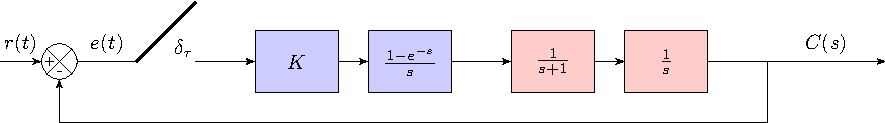
\includegraphics[width=1\linewidth]{samplerTesting-cropped.pdf}
\end{minipage}
\begin{align*}
& G(z) = \mathcal{Z} \left\{\left(\frac{1-e^{-s}}{s}\right) \left[ \frac{1}{s+1}\right] \left[\frac{1}{s}\right] \right\} \rightarrow G_1(z) = (1-z^{-1})\mathcal{Z} \left\{ G_{rest}(s) \right\}
\end{align*}
\begin{minipage}[h]{0.65\linewidth}
%\medbreak\noindent\minipage{\columnwidth}
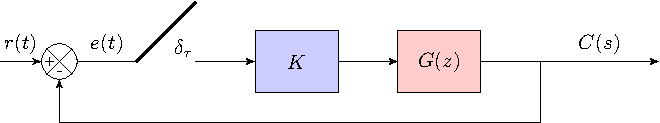
\includegraphics[width=1.05\linewidth]{sampleEND-cropped.pdf}%\endminipage\medbreak
\end{minipage}
\begin{minipage}[h]{0.35\linewidth}
\[
G(z) = \frac{ze^{-1}+(1-ze^{-1})}{(z-1)(z-e^{-1})} 
\]
\end{minipage}
$$ \text{ZOH(zero-hold-system)} \quad 
f^\ast(t) = \sum_{k=-\infty}^\infty f(kT)\delta(t-kT)  \quad 
G_{h}(s)= \frac{1-e^{-Ts}}{s}
$$
\subsection{Stability Test for Digital Systems}
\vspace*{-0.45cm}
\begin{align*}
& P(z) = a_0z^n+a_1z^{n-1} + \cdots + a_{n-1}z+a_n \quad G(z)= \frac{A(z)}{P(z)} \\
& \text{Stability Condition:} \quad P(z) \neq 0 \quad |z| \geq 1 \quad (\text{Draw Unit Circle to test stability})\\
& \text{Routh-Stability in Digital Domain: } s = \frac{z+1}{z-1} \quad z=\frac{s+1}{s-1}
\end{align*}
%\begin{table}
%\captionof{Table}{Jury-Marden Table}
\textbf{Jury-Marden Table Uses function P of z} \newline
%\vspace*{-0.25cm}
\begin{minipage}[t]{1\linewidth}
\begin{minipage}[h]{0.25\linewidth}
\begin{align*}
& b_k = \det \begin{bmatrix}
a_n & a_{n-1-k} \\
a_0 & a_{k+1}
\end{bmatrix} \\
& k = 0,1,  \cdots n-1 \\
& c_k = \det \begin{bmatrix}
b_{n-1} & b_{n-2-k} \\
b_0 & b_{k+1}
\end{bmatrix} \\
& k = 0,1,  \cdots n-1 \\
& q_k = \det \begin{bmatrix}
p_{3} & p_{2-k} \\
p_0 & p_{k+1}
\end{bmatrix} \\
& k =0,1,2
\end{align*}
\end{minipage}
\begin{minipage}[h]{0.75\linewidth}
\begin{tabular}{llllllll}
%\cline{1-5}
Row & $z^0$     & $z^1$     & $z^2$     &          & $z^{n-2}$ & $z^{n-1}$ & $z^n$ \\ %\cline{1-5}
1   & $a_n$     & $a_{n-1}$ & $a_{n-2}$ & $\cdots$ & $a_2$     & $a_1$     & $a_0$ \\
2   & $a_0$     & $a_1$     & $a_2$     & $\cdots$ & $a_{n-2}$ & $a_{n-1}$ & $a_n$ \\
3   & $b_{n-1}$ & $b_{n-2}$ & $b_{n-3}$ & $\cdots$ & $b_1$     & $b_0$     &       \\ %\cline{1-5}
4   & $b_0$     & $b_1$     & $b_2$     & $\cdots$ & $b_{n-2}$ & $b_{n-1}$ &       \\
5   & $c_{n-2}$ & $c_{n-3}$ & $c_{n-4}$ & $\cdots$ & $c_0$     &           &       \\
6   & $c_0$     & $c_1$     & $c_2$     & $\cdots$ & $c_{n-2}$ &           &      \\
2n-5& $p_3$ & $p_2$ & $p_1$ & $p_0$ & & \\
2n-4& $p_0$ & $p_1$ & $p_2$ & $p_3$ & & \\
2n-3& $q_2$ & $q_1$ & $q_0$ & & & 
\end{tabular}
\end{minipage}
\end{minipage}

\textbf{Necessary and Sufficient Condition for Stability} \newline
\begin{minipage}[h]{0.55\linewidth}
\begin{enumerate}
\item $|a_n| < |a_0|$ 
\item $P(1) > 0$
\item \begin{align*}
P(-1) & > 0 \ \text{for n even } \\
& < 0 \ \text{for n odd}
\end{align*}
\item $b_{n-1}> |b_0|, |c_{n-2}|>|c_0|, \cdots |q_2| > |q_0|$
\end{enumerate}
\end{minipage}
\begin{minipage}[h]{0.5\linewidth}
\textbf{Special Case n =2} \newline 
$P(z) =a_0z^2+a_1z+a_2$ \newline 
\begin{tabular}{c c c}
$z^0$ & $z^1$& $z^2$ \\
$a_2$ & $a_1$ & $a_0$
\end{tabular} \newline
$P(z) \neq 0$ for $|z| \geq 1$ if and only if 
\begin{enumerate}
\item $|a_2| < |a_0|$
\item $P(1) > 0$
\item $P(-1) > 0 \quad (n=2)$
\end{enumerate}
\end{minipage}

\textbf{Root Locus} presents the poles of the closed loop system when the gain K changes from zero to infinity.

\textbf{Construction of the Root Locus}

Open loop transfer function
$ \displaystyle \text{KH}\left( s \right)G\left( s \right) = K\frac{B(s)}{A(s)}$

m: the order of the \textbf{open-loop} numerator polynomial.

n: the order of the \textbf{open-loop} denominator polynomial. $q=n-m$

\textbf{Rule 1:} number of branches equals the number of poles of the
 open-loop transfer function

\textbf{Rule 2:} If the total number of poles and zeros of the open-loop
 system to the right of the s-point on the real axis is odd, then this
 point lies on the locus.

\textbf{Rule 3:} The locus starting point (K=0) are at the open-loop
poles and the locus ending points (K=$\infty$) are at the open loop zeros and
n-m branches terminate at infinity.

\textbf{Rule 4 and 5:} Slope of asymptotes of root locus as `s' approaches infinity. \newline Abscissa of the intersection between asymptotes of root locus and real-axis.
\[\sigma  = {\frac{\sum\limits_{i = 1}^n {{p_i}}  - \sum\limits_{i = 1}^m {{z_i}} }{q}} \quad \theta = \pm r{\frac{180}{q}} \quad \text{where r=1, 3, 5} \]

%\textbf{Rule 5:} 

\textbf{Rule 6:} Break-away and break-in points. From the characteristic
equation

\[f\left( s \right) = A\left( s \right) + KB\left( s \right) = 0\ \ \ \ and\ \ \ \ K = - \frac{A\left( s \right)}{B\left( s \right)}\]

The break-away and break-in points can be found from

\[\frac{\text{dK}}{\text{ds}} = - \frac{A^{'}\left( s \right)B\left( s \right) - A\left( s \right)B^{'}\left( s \right)}{B^{2}\left( s \right)} = 0
\]

\textbf{Rule 7:} Angle of departure from complex poles or zeros.
Subtract from $180^o$ the sum of all angles from all other zeros and poles
of the open-loop system to the complex pole (or zero) with appropriate signs. 

\[ \text{Z-transform: Definition} \quad F(z)=Z[f(t)]-Z[f(kT)]=\sum_{k=0}^{\infty}f(kT)z^{-k}\]
\end{multicols}
\newpage
\begin{multicols}{3}
\begin{align*}
& e^\ast(\infty)=\lim_{z \rightarrow 1} (1-z^{-1})E(z) \\
& K_p=\lim_{z \rightarrow 1} G(z), \quad e^\ast (\infty) = \frac{1}{1+K_p} \\
& e^\ast(\infty) = \frac{1}{K_v}, \quad K_v = \frac{1}{T} \lim_{z \rightarrow 1}(z-1) G(z)  \\
& e^\ast(\infty) = \frac{1}{K_a}, \quad K_a = \frac{1}{T^2} \lim_{z \rightarrow 1}(z-1)^2 G(z)
\end{align*}

{\bf Linear Factor Rule.}  
For each factor of $Q$ of the form $(ax+b)^m$, 
the partial fraction decomposition contains 
the following sum of $m$ partial fractions:  
\[
\frac{A_1}{ax+b} + \frac{A_2}{(ax+b)^2} + \cdots + \frac{A_m}{(ax+b)^m},
\]
where the $A_i$ are constants to be determined.  

\medskip
\noindent
{\bf Quadratic Factor Rule.}  
For each factor of $Q$ of the form $(ax^2+bx+c)^m$, 
where $ax^2+bx+c$ is an irreducible quadratic, 
the partial fraction decomposition contains 
the following sum of $m$ partial fractions:  
\[
\frac{A_1x+B_1}{ax^2+bx+c} + \frac{A_2x+B_2}{(ax^2+bx+c)^2} + \cdots 
  + \frac{A_mx+B_m}{(ax^2+bx+c)^m},
\]
where the $A_i$ and $B_i$ are constants to be determined. 
\begin{align*}
& x(k+2)-\frac{3}{2}x(k+1)+\frac{1}{2}x(k)=u(k), \text(x(0)=1,x(1)=5/2) \\
& [z^2X(z)-z^2x(0)-zx(1)]-\frac{3}{2}(zX(z)-zx(0)]+\frac{1}{2}X(z)=\frac{z}{z-1} \\
& [z^2-1.5z+0.5z]X(z)= \frac{z}{z-1}+z^2+(2.5-1.5)z \\
& X(z) = \frac{z[1+(z+1)(z-1]}{(z-1)(z-1)(z-0.5)}=\frac{z^3}{(z-1)^2(z-0.5)} \\
& \frac{X(z)}{z}=\frac{z^2}{(z-1)^2(z-0.5)}=\frac{A_{11}}{(z-1)^2}+\frac{A_{12}}{z-1}+\frac{A_{13}}{z-0.5}
\end{align*}
Geometric Sum $\sum\limits_{k = -N}^{N} {ar^{k - 1} = a\frac{1-r^{N}}{{1 - r}}} \sum_{i=0}^\infty a^i=\frac{1}{1-a}$
\textbf{Example Partial Fractions}
\begin{align*}
& \frac{20}{\left(s+3\right)\,\left(s^2+6\,s+25\right)} \rightarrow 
\frac{5}{4\,\left(s+3\right)}-\frac{\frac{5\,s}{4}+\frac{15}{4}}{s^2+6\,s+25} \\
& \frac{5\,z}{4\,\left(z-{\mathrm{e}}^{-3}\right)}+\frac{5\,z\,{\mathrm{e}}^3\,\left(\cos\left(4\right)-z\,{\mathrm{e}}^3\right)}{4\,\left({\mathrm{e}}^6\,z^2-2\,\cos\left(4\right)\,{\mathrm{e}}^3\,z+1\right)} \ \text{Z-table} = \text{17}
\end{align*}
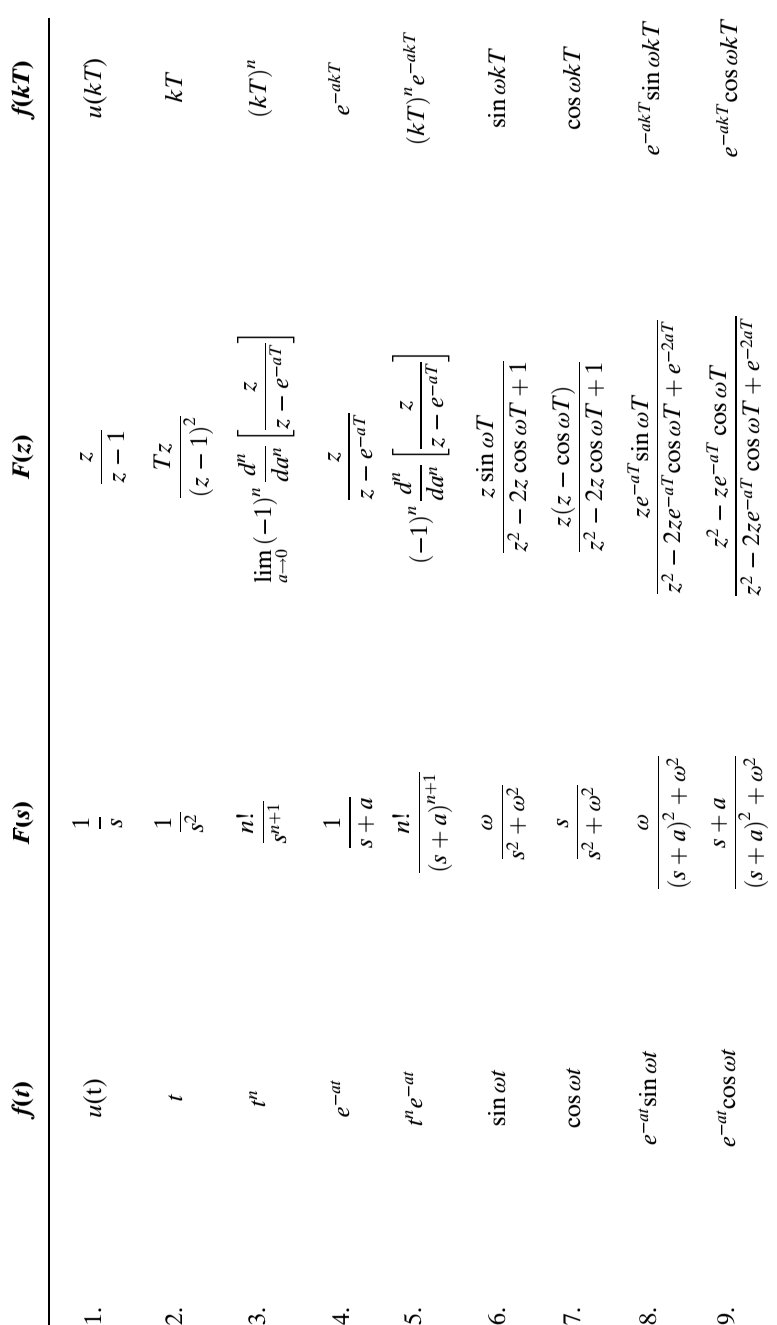
\includegraphics[width=1\linewidth]{NICEPictureRotate.png}
$\text{Ch.eqn} =\Delta P(z)=z^2+(K-4)z+0.8=0$ \newline
Inputting $z=1 \text{ and } z=-1$, $K=-0.8-1+4=2.2$, $K=(1)^2+4+0.8=5.8$, for stability $-1<K<1$.
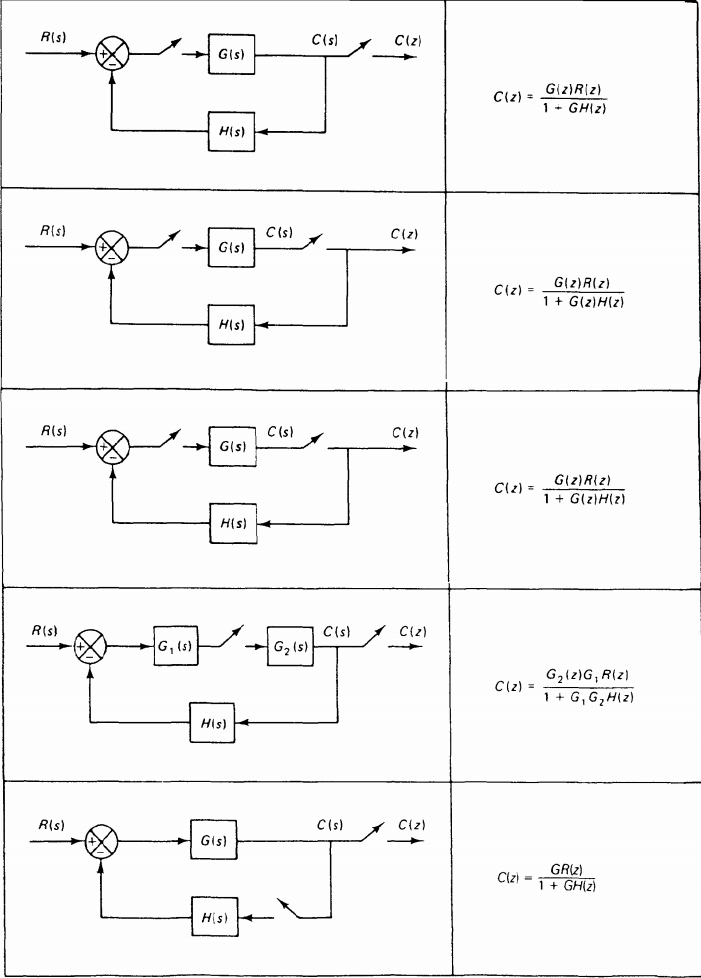
\includegraphics[width=1\linewidth]{OgataTable.png}
% \begin{align*}
% & G_p(s)=\frac{K}{s(s+3)} \rightarrow \frac{1}{s(s+3)}
% \end{align*}
%https://www.wolframalpha.com/input/?i=Plot++(t-2)*heaviside(t-2)-+(t-5)*heaviside(t-5)
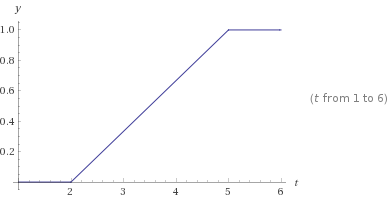
\includegraphics[width=1\linewidth]{heavsidePlot.png}
\begin{align*}
& \frac{1}{3}((t-2)u(t-2)- (t-5)u(t-5)) \rightarrow \frac{z^2 + z + 1}{3 (z - 1) z^4} \\
& =
\frac{1(z^{-3}+z^{-4}+z^{-5})}{3(1-z^{-1})} \quad \frac{1}{3}z^{-3}+\frac{2}{3}z^{-4}+z^{-5}+z^{-6}+ \cdots 
\end{align*}
\end{multicols}

\newpage
\begin{sidewaysfigure}
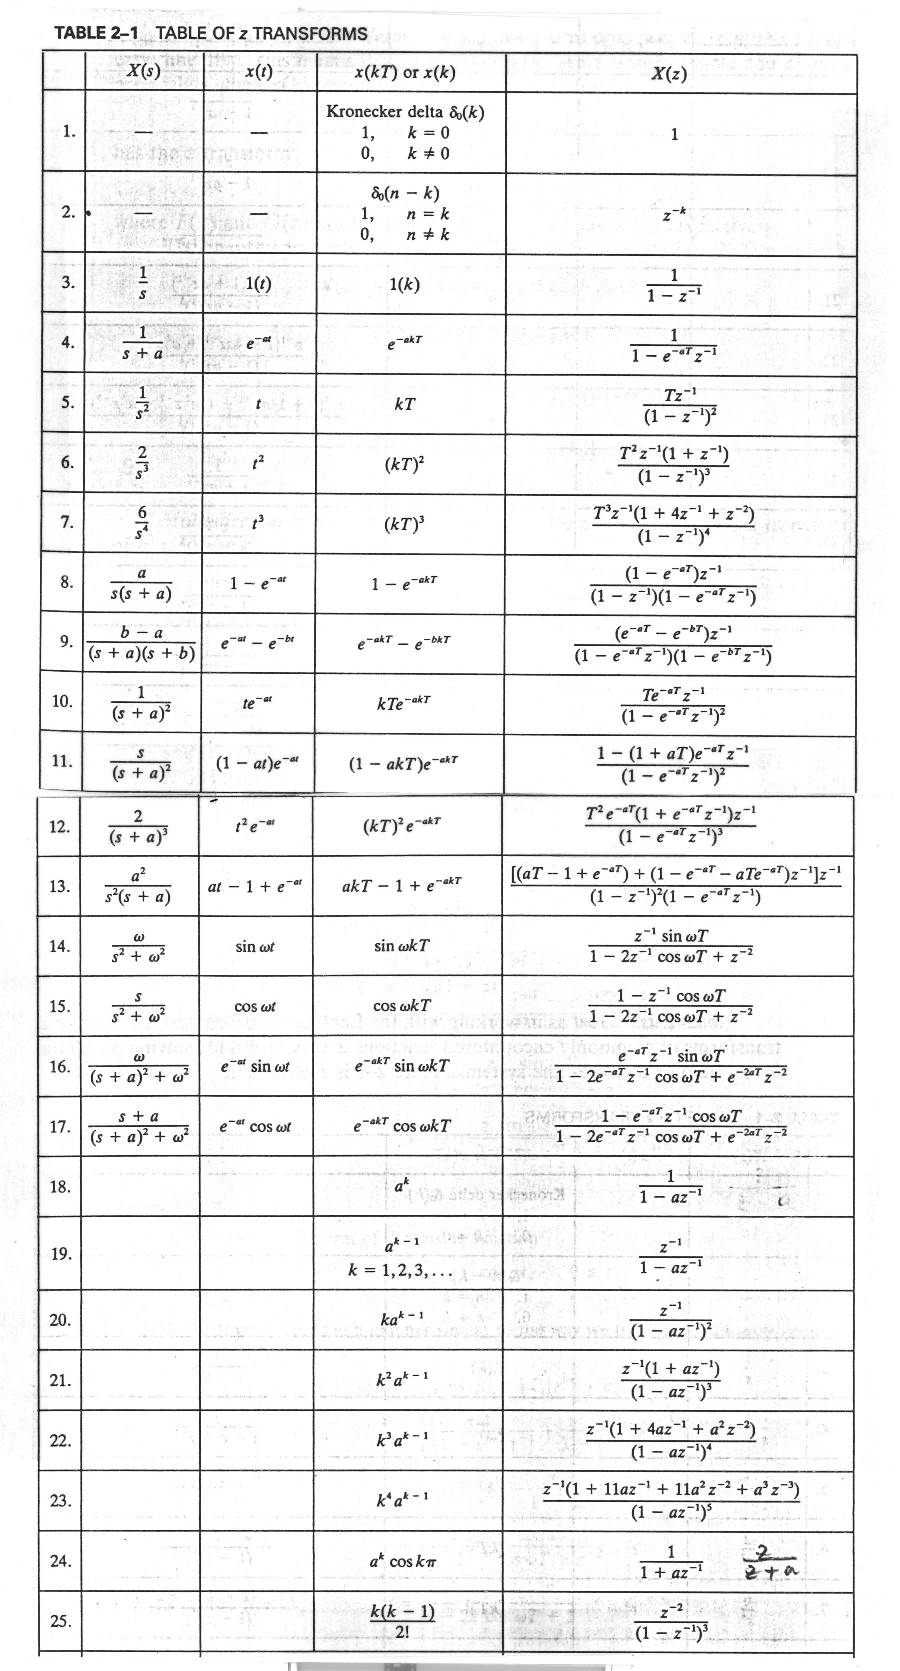
\includegraphics[width=0.75\linewidth]{Table_z_Transforms.pdf}
\end{sidewaysfigure}
%\end{table}


\textbf{Necessary and Sufficient Condition for Stability} \newline

\begin{enumerate}
\item $|a_n| < |a_0|$ 
\item $P(1) > 0$
\item \begin{align*}
P(-1) & > 0 \ \text{for n even } \\
& < 0 \ \text{for n odd}
\end{align*}
\item $b_{n-1}> |b_0|, |c_{n-2}|>|c_0|, \cdots |q_2| > |q_0|$
\end{enumerate}

\textbf{Special Case n =2} \newline 
$P(z) =a_0z^2+a_1z+a_2$ \newline 
\begin{tabular}{c c c}
$z^0$ & $z^1$& $z^2$ \\
$a_2$ & $a_1$ & $a_0$
\end{tabular} \newline
$P(z) \neq 0$ for $|z| \geq 1$ if and only if 
\begin{enumerate}
\item $|a_2| < |a_0|$
\item $P(1) > 0$
\item $P(-1) > 0 \quad (n=2)$
\end{enumerate}

 \textbf{Root Locus} presents the poles of the closed loop system when the gain K changes from zero to infinity.

 \textbf{Construction of the Root Locus}

 Open loop transfer function
 $ \displaystyle \text{KH}\left( s \right)G\left( s \right) = K\frac{B(s)}{A(s)}$

m: the order of the \textbf{open-loop} numerator polynomial.

 n: the order of the \textbf{open-loop} denominator polynomial. $q=n-m$

 \textbf{Rule 1:} number of branches equals the number of poles of the
 open-loop transfer function

 \textbf{Rule 2:} If the total number of poles and zeros of the open-loop
 system to the right of the s-point on the real axis is odd, then this
 point lies on the locus.

\textbf{Rule 3:} The locus starting point (K=0) are at the open-loop
 poles and the locus ending points (K=$\infty$) are at the open loop zeros and
 n-m branches terminate at infinity.

\textbf{Rule 4 and 5:} Slope of asymptotes of root locus as `s' approaches infinity. \newline Abscissa of the intersection between asymptotes of root locus and real-axis.
\begin{align*}
& \sigma  = {\frac{\sum\limits_{i = 1}^n {{p_i}}  - \sum\limits_{i = 1}^m {{z_i}} }{q}} \quad \theta = \pm r{\frac{180}{q}} \quad \text{where r=1, 3, 5} \\
& f\left( s \right) = A\left( s \right) + KB\left( s \right) = 0\ \ \ \ and\ \ \ \ K = - \frac{A\left( s \right)}{B\left( s \right)} \\
& \frac{\text{dK}}{\text{ds}} = - \frac{A^{'}\left( s \right)B\left( s \right) - A\left( s \right)B^{'}\left( s \right)}{B^{2}\left( s \right)} = 0 \\
 \end{align*}
 \textbf{Rule 5:} 

 \textbf{Rule 6:} Break-away and break-in points. From the characteristic
  equation

  \[f\left( s \right) = A\left( s \right) + KB\left( s \right) = 0\ \ \ \ and\ \ \ \ K = - \frac{A\left( s \right)}{B\left( s \right)}\]

  The break-away and break-in points can be found from

  \[\frac{\text{dK}}{\text{ds}} = - \frac{A^{'}\left( s \right)B\left( s \right) - A\left( s \right)B^{'}\left( s \right)}{B^{2}\left( s \right)} = 0 \]

  \textbf{Rule 7:} Angle of departure from complex poles or zeros.
  Subtract from $180^o$ the sum of all angles from all other zeros and poles
  of the open-loop system to the complex pole (or zero) with appropriate signs. 

 \begin{align*}
& \text{Z-transform: Definition} \quad F(z)=Z[f(t)]-Z[f(kT)]=\sum_{k=0}^{\infty}f(kT)z^{-k} \\
& e^\ast(\infty)=\lim_{z \rightarrow 1} (1-z^{-1})E(z) \quad K_p=\lim_{z \rightarrow 1} GH(z), \quad e^\ast (\infty) = \frac{1}{1+K_p} \\
& e^\ast(\infty) = \frac{1}{K_v}, \quad K_v =  \lim_{z \rightarrow 1} \frac{(1-z^{-1}) GH(z)}{T}  \\
& e^\ast(\infty) = \frac{1}{K_a}, \quad K_a =  \lim_{z \rightarrow 1}\frac{(1-z^{-1})^2 GH(z)}{T^2}
\end{align*}

{\bf Linear Factor Rule.}  
 For each factor of $Q$ of the form $(ax+b)^m$, 
 the partial fraction decomposition contains 
 the following sum of $m$ partial fractions:  
\[
\frac{A_1}{ax+b} + \frac{A_2}{(ax+b)^2} + \cdots + \frac{A_m}{(ax+b)^m},
\]
 where the $A_i$ are constants to be determined.  

\medskip
\noindent
{\bf Quadratic Factor Rule.}  
 For each factor of $Q$ of the form $(ax^2+bx+c)^m$, 
 where $ax^2+bx+c$ is an irreducible quadratic, 
% the partial fraction decomposition contains 
 the following sum of $m$ partial fractions:  
\[
\frac{A_1x+B_1}{ax^2+bx+c} + \frac{A_2x+B_2}{(ax^2+bx+c)^2} + \cdots 
  + \frac{A_mx+B_m}{(ax^2+bx+c)^m},
\]
 where the $A_i$ and $B_i$ are constants to be determined. 


Geometric Sum $\sum\limits_{k = -N}^{N} {ar^{k - 1} = a\frac{1-r^{N}}{{1 - r}}} \sum_{i=0}^\infty a^i=\frac{1}{1-a}$

$ x(k+2)-\frac{3}{2}x(k+1)+\frac{1}{2}x(k)=u(k), \text(x(0)=1,x(1)=5/2) $

$[z^2X(z)-z^2x(0)-zx(1)]-\frac{3}{2}(zX(z)-zx(0)]+\frac{1}{2}X(z)=\frac{z}{z-1}$


\textbf{Effects of T on Transient Behaviour} \hfill \break 
$s= -\zeta \omega_n \pm j \omega_n \sqrt{1-\zeta^2}$,  \hfill \break 
$\zeta$: damping ratio  \hfill \break 
$\omega_n$: undamped natural frequency,  \hfill \break 
$\omega_d$: damped natural frequency \hfill \break
$z=e^{Ts} \rightarrow z= \exp\left[T(-\zeta \omega_n +j\omega_n \sqrt{1-\zeta^2})\right]$, and
$|z|=e^{-T \zeta \omega_n}$, $\angle z = T \omega_n \sqrt{1-\zeta^2}= T \omega_d$. $\uparrow T$ makes system less stable (for the same gain K) than $\downarrow T$.
\textbf{Matrix Inverses for 2x2 and 3x3}
\begin{align*}
& A^{-1} = \begin{bmatrix}
a & b \\
c & d
\end{bmatrix}^{-1}= \frac{1}{|A|}\begin{bmatrix}
d & -b \\
-c & a
\end{bmatrix} \ \begin{bmatrix}
a & b & c \\
d & e & f \\
g & h & i
\end{bmatrix}^{-1} \\
& A^{-1} = 
\frac{1}{|A|}\begin{bmatrix}
% Row one determinate
+\begin{vmatrix}
e & f \\
h & i
\end{vmatrix} & 
-\begin{vmatrix}
b & c \\
h & i
\end{vmatrix} & 
+\begin{vmatrix}
b & c \\
e & f
\end{vmatrix} \\
& & \\
-\begin{vmatrix}
d & f \\
g & i
\end{vmatrix} & +\begin{vmatrix}
a & c \\
g & i
\end{vmatrix} &
-\begin{vmatrix}
a & c \\
d & f
\end{vmatrix} \\
& & \\
+\begin{vmatrix}
d & e \\
g & h
\end{vmatrix} &
-\begin{vmatrix}
a & b \\
g & h
\end{vmatrix} &
+\begin{vmatrix}
a & b \\
d & e
\end{vmatrix}
\end{bmatrix}^{-1}
\end{align*}
\textbf{Bilinear Transform}  \hfill \nopagebreak
$s= \frac{2(1-z^{-1})}{T(1+z^{-1})}$, $z=\cfrac{1+0.5Ts}{1-0.5Ts}$.

\text{1. Stability} $\Re[s] < 0$

$\displaystyle \Re \left(\frac{2}{T} \frac{1-z^{-1}}{1+z^{-1}}\right)= \Re \left(\frac{2}{T}\frac{z-1}{z+1}\right) < 0$, $z= \sigma + j \omega$ \hfill \nopagebreak

$\displaystyle \Re \frac{z-1}{z+1}=\Re \left[\frac{\sigma^2-1+\omega^2+2j\omega}{(\sigma+1)^2+\omega^2}\right] \rightarrow \sigma^2-1+\omega^2 < 0$.


\textbf{Solution of inhomogeneous state equations}
scalar $\dot{x}=ax+bu \quad \dot{x}-ax=bu$
\begin{align*}
& e^{-at}[\dot{x}(t)-ax(t)]=\underbrace{\frac{d}{dt}[e^{-at}x(t)]=e^{-at}bu(t)}_{\text{integrate ~$0 \rightarrow t$}} \\
& e^{-at}x(t)-x(0) = \int^t_0 e^{-a \tau}bu(\tau) d\tau \\
& \rightarrow x(t)=e^{at}x(0)+e^{at}\int_0^te^{-a\tau}bu(\tau)d\tau
\end{align*}
matrix: $\dot(x)=Ax+bu$, but taking $\mathcal{L}^{-1}$ leads to  \hfill \break  $x(t)=e^{At}x(0)+\int_{0}^{t}e^{A(t-\tau)}bu(\tau) d\tau$

\textbf{Controllable Canonical Form} \hfill \nopagebreak

% \hfill \break \nopagebreak
\resizebox{.9\linewidth}{!}{
  \begin{minipage}{\linewidth}
\begin{align*}
& G(z) = \frac{b_0+b_1z^{-1}+ \cdots + b_nz^{-n}}{1+a_1z^{-1}+ \cdots + a_n}= \frac{b_0z^n+b_1z^{n-1}+ \cdots + b_n}{z^n+a_1z^{n-1}+\cdots + a_n} \\
& G(z)= b_0 + \frac{(b_1-a_1b_0)z^{-1}+(b_2-a_2b_0)z^{-2}+ \cdots + (b_n-a_nb_0)z^{-n-1}}{1+a_1z^{-1}+a_2z^{-2}+ \cdots + a_nz^{-n}} \\
& \begin{bmatrix}
x_1(k+1) \\
 \vdots \\
x_n(k+1)
\end{bmatrix}= \begin{bmatrix}
0      & 1         & 0      & \cdots \\
\vdots & \cdots    &        & \vdots \\
\vdots &           &  \cdots      &   1    \\
-a_n   &  \cdots   & \cdots & -a_1
\end{bmatrix}\begin{bmatrix}
x_1(k) \\
 \vdots \\
x_n(k)
\end{bmatrix}+\begin{bmatrix}
0 \\
 \vdots \\
0 \\
1
\end{bmatrix}u(k) \\
& y(k) = \begin{bmatrix}
b_n-a_nb_0, & b_{n-1}a_{n-1}b_0, & b_1-a_1b_0
\end{bmatrix} \begin{bmatrix}
x_1(k) \\
\vdots \\
x_n(k)
\end{bmatrix} + b_0 u(k) \\
& z \rightarrow s \quad  zX(z) = \mathcal{Z}[x(k+1)] \quad  sX(s) = \mathcal{L}[x(t)]
\end{align*}
  \end{minipage}
} \hfill \nopagebreak

\textbf{Observable Canonical Form} \hfill \nopagebreak

\resizebox{.9\linewidth}{!}{
  \begin{minipage}{\linewidth}
\begin{align*}
& \begin{bmatrix}
\dot{x_1} \\
 \vdots \\
\dot{x_n}
\end{bmatrix}= \begin{bmatrix}
0      & 0         & 0      & -a_n     \\
1 & \cdots    &        & -a_{n-1} \\
0 &           & \cdots &   \vdots \\
0   &  0   & 1 & -a_1
\end{bmatrix} \begin{bmatrix}
x_1 \\
 \vdots \\
x_n
\end{bmatrix}+\begin{bmatrix}
b_n-a_nb_0 \\
 \vdots \\ 
b_1-a_1b_0
\end{bmatrix}u(k) \\
& y(k) = \begin{bmatrix}
0, & \cdots & \cdots, & 0, & 1 
\end{bmatrix} \begin{bmatrix}
x_1 \\
\vdots \\
x_n
\end{bmatrix} + b_0 u(k) 
\end{align*}
  \end{minipage}
} \hfill \nopagebreak

\textbf{Part-Frac-Expansion Method, Dia Canonical} %\hfill \nopagebreak
\vspace{-0.425cm}
\begin{align*}
& G(z) =  b_0 + \frac{c_1}{z-p_1} + \cdots \ \cdots + \frac{c_n}{z-p_n} \\
& \begin{bmatrix}
x_1(k+1) \\
\vdots \\
\vdots \\
x_n(k+1)
\end{bmatrix} =  \begin{bmatrix}
p_1     & 0       & \cdots  & 0      \\
0       & \vdots  &         & 0      \\
\vdots  &         &  \vdots & \vdots \\
0       & 0       &  \cdots & p_n
\end{bmatrix}\begin{bmatrix}
x_1(k) \\
\vdots \\
\vdots \\
x_n(k)
\end{bmatrix} + \begin{bmatrix}
1 \\
1 \\
\vdots \\
1
\end{bmatrix} u(k) \\
&  y(k) = \begin{bmatrix}
c_1 & \cdots & c_n
\end{bmatrix} \begin{bmatrix}
x_1    \\
\vdots \\
x_n
\end{bmatrix} + b_0 u(k)
\end{align*}

\textbf{Special Case} %hill \nopagebreak
%
\vspace{-0.425cm}
\begin{align*}
& y^{(n)}+a_1y^{(n-1)}+ \cdots + a_{n-1}y+a_{n}=u \quad \dot{x} = Ax + bu  \\
& x = \begin{bmatrix}
x_1 \\
\vdots \\
\vdots \\
x_n
\end{bmatrix} \quad 
A = \begin{bmatrix}
0      & 1        &  \vdots & \vdots       & 0        \\
0      & 0        &  1      &              & \vdots   \\
\vdots &          &         & \ddots       & \vdots   \\
0      &          &         &              &  1       \\
-a_n   & -a_{n-1} &  \cdots & \cdots       & -a_1 
\end{bmatrix}
\end{align*}

\vspace*{-0.90cm}

\begin{minipage}[h]{0.25\linewidth}
\[
b = \begin{bmatrix}
0 \\
0 \\
\vdots \\
1
\end{bmatrix}
\]
\end{minipage}
\begin{minipage}[h]{0.75\linewidth}
\begin{align*}
& c = [1 \ 0 \ .. \ 0] \ \quad y =cx+du \ \text{and} \ d=0 \\
& Y(s) = [c(sI-A)^{-1}b+d]U(s) \quad \\ 
& \frac{Y(z)}{U(z)} = c(zI-A)^{-1}b+d 
\end{align*}
\end{minipage}
\textbf{Deadbeat Controller and Deadbeat Response}
\vspace*{-0.25cm}
\begin{align*}
& x(k+1)=Gx(k)+Hu(k) \quad u(k)=-Kx(k) \\
& x(k+1)=(G-HK)x(k) \quad x(k)=(G-HK)^kx(0) \\
& x(k) = (G-HK)^kx(0) \quad x(k) =0 \quad \text(for) k \geq \quad q (q \leq n) \\
& \det(zI-G+HK)=z^n \quad N^n =0, \text{N is nilpotent matrix.}
\end{align*}
\vspace*{-0.7cm}

\textbf{Controllability} A system is controllable, if and only if, it is possible to transfer the system state from any arbitrary initial state x(0) to the origin in finite time. initial state x(0) $\rightarrow$ desired state: x(n)=0.%
%
\textbf{Controllability condition for SI continuous systems:} $\det C = \det[b, \ \ Ab, \ \, \cdots, A^{n-1}b] \neq 0$.

\textbf{Observability} A system is observable if any initial state x(0) can be determined from a finite number of output observations. $\det O_c = \det \begin{bmatrix} 
c \\ cA \\ \vdots \\ cA^{n-1} \end{bmatrix} \neq 0$.

\textbf{Continuous State Transition Matrix:} $\phi(t)$,
$\phi(t)=e^{At}= \mathcal{L}^{-1}[(sI-A)^{-1}]$, then $\dot{\phi}(t)=A\phi(t) \quad \phi(0)=I$, $\dot(x)=Ax$ %\hfill \linebreak

Verification: $x(t)=\phi(0)x(0)=Ix(0)$ 
$\dot{x}(t)=\dot{\phi}(t)x(0)=A\phi(t)x(0)=Ax(t)$. 

Properties of $\phi(t)$:
\vspace*{-0.4cm}
\begin{align*}
& 1) \ \ \phi(0)=e^{A0}=I \\
& 2) \ \ \phi(t) = e^{At} = (e^{(-At)})^{-1}=[\phi(-t)]^{-1} \\
& 3) \ \ \phi(t_1+t_2)=\phi(t_1)\phi(t_2)=\phi(t_2)\phi(t_1) \\
& 4) \ \ [\phi(t)]^n = \phi(nt) \\
& 5) \phi(t_0-t_1)\phi(t_1-t_2)=\phi(t_0-t_2)=\phi(-t_1+t_0)\phi(-t_2+t_1) \\
& e^{A(t_0-t_1)}e^{A(t_1-t_2)} = e^{A(t_0-t_2)}=e^{-A(t_1-t_0)}e^{-A(t_2-t_1)}
\end{align*}%
%
\textbf{BIBO Stability}
Output is bounded for any bounded input.
CTS systems : Poles in left half plane, Discrete Systems: poles inside unit circle.

\textbf{INTERNAL ( Also asymptotic stability)}
Def: Equilibrium state:
 Continuous systems: Assume u(t) = 0;
 $\dot{x}_e=0=Ax_e+bu \rightarrow x_e=0$ \hfill \break 
  Discrete systems: Assume u(k) = 0;
 $x_e(k+1)=0=x_e(k)+Gx_e(k) \rightarrow x_e=0$ \hfill \break
\textbf{Def:} A system is asymptotically stable if any initial condition x(0) converges to
the equilibrium state $x_e=0$.
 (It is assumed $u(t) = 0,t \leq0$  or $u(k)=0, k\geq 0$)
 
 \textbf{Condition for asymptotic stability}: \hfill \break CTS $\Re[\lambda_i\{A\}]<0$ \hfill \break Discrete $|\lambda_i 
 \{G\}|$
, all eigenvalues in unit circle

%\newpage 
%\begin{multicols}{3}

$\text{BIBO Stability} \rightarrow \text{Asymptotic Stability (AS)}$ \hfill \break
BIBO Stability \& no pole zero cancellation $\rightarrow $ AS \hfill \break 
%
Eigenvalues of A are the solutions of $\det(I\lambda -A) = 0$, \hfill \break
Poles of G(z) are the zeros of denominator poly. 
$G(z)=d+c(zI-A)^{-1}b$ where $(zI-A)^{-1}=\frac{\text{adj}(zI-A)}{\text{det}(zI-A)}$
% $A_{ij}=(-1)^{i+j} M_{ij}$, (minor $M_{ij}$, $\det$ with deleted i and j rows/col.
% adj A
C: nonsingular if system controllable. If the system is controllable,
any closed-loop poles can be obtained, %i.e any desired transient response characteristics can be obtained
%\begin{comment}
%Adding a comment here, make sure to add in information about the controlleres and go home and study tommorw
%\end{comment}

\textbf{Feed-forward observers} State Observer: $\tilde{X}(k+1)=G\tilde{x}(k)+Hu(k)$
$\tilde{y}(k)=c \tilde{x}(k)$, Observed state: $\tilde{x}(k)$, Observation error: $e(k)=x(k)-\tilde{x}(k)$, $e(k+1)=Ge(k)$, Dynamics of error depend on G \hfill \break 
\textbf{Prediction (full order) observer} where the estimate $\bar{x}(k+1)$ is obtained based on measurements of up to y(k).
\vspace*{-0.2cm}
\begin{align*}
& \bar{x}(k+1)=G\bar{x}(k)+Hu(k)+k_e[y(k)-\bar{y}(k)] \\
& \bar{x}(k+1)=[G-k_e c] \tilde{x}(k)+Hu(k)+k_ecx(k)
\end{align*}
$k_e$ for this observer can be obtained 
using $k_e=O^{-1}\bar{A}^{-1}(\alpha-a)^T$, where \hfill \break 
$\tilde{A}=\begin{bmatrix}
1   & 0 \cdots & \cdots & 0 \\
a_1 & 1 & & \\
\vdots & a_1 & . &  \\
\vdots & . & . & \\
a_{n-1} & a_{n-2} & \cdots & a_1 & 1
\end{bmatrix}$, \hfill \break  lower triangular Toeplitz matrix, A square matrix that is not singular, i.e., one that has a matrix inverse.
\textbf{Current observer} where the estimate is obtained based on measurements
up to $y(k+1)$.
\vspace*{-0.15cm}
\begin{align*}
& \tilde{x}(k+1)=G\tilde{x}(k)+Hu(k)+K_e[y(k+1)-c\tilde{x}(k+1)] \\
& \bar{z}(k+1)=c\bar{x}(k+1)
\end{align*}
\vspace*{-0.15cm}
\textbf{ASYMPTOTIC OBSERVERS 4 CTS
SYS} 
\vspace*{-0.15cm}
\begin{align*}
& \dot{x}(t) = A x(t)+bu(t) \quad x(0-)=x_0 \\
& y(t) = cx(t) \quad t > 0- \\
& O x(0-) = [y(0-), \ \cdots \ y^{n-1}(0-)]
\end{align*}
\textbf{Open-loop Observer}
Use ($\{A,B,c\}$, $\{u(t), t> 0\}$, and $x_0$) $\rightarrow \{x(t),t>0-\}$,

Effects of disturbance $\epsilon$:
$\tilde{x}_0=x_0-\epsilon$, $|\epsilon| \ll |x_0|$, $\tilde{\dot{x}}(t)=A \tilde{x}(t)+bu(t)$, $\tilde{x}(0-)=\tilde{x}_0=x_0-\epsilon$,
$\dot{e}(t)=Ae(t)$, $e(0-)=\epsilon$, A is unstable $e(t) \rightarrow \infty$

\textbf{Closed-loop observer:}
Output Error: $y(t)-\tilde{y}(t)=y(t)-c\tilde{x}(t)=c[x(t)-\tilde{x}(t=ce(t)$, Observer $\tilde{x}(t)=A \tilde{x}(t)+bu(t)+l[y(t)-c\tilde{x}(t)$, $\tilde{x}(t_o)=\tilde{x}_o$ $\tilde{x}_o$ an estimated initial state vector $l$: feedback gain vector.
\textbf{Observer design:}
$l=O^{-1}\tilde{A}^{-1}(\alpha-a)^T$ \hfill \break 
%$\det C = \det[H, \ GH, \ G^2H, \ \cdots, \ G^{n-1}H] \neq 0$, \\ \hfill
%$O_d = \begin{bmatrix}
%c & cG & \vdots & cG^{n-1}
%\end{bmatrix}^T$
%$\dot{\hat{x}}=T^{-1}AT\hat{x} + T^{-1}Bu$, $x = T\hat{x}$,$T=MW$, control matrix $M$, W is like $\tilde{A}$,but with upper triangular Toeplitiz matrix. $Q = (WN\ast)^{-1}$, N is observability matrix, and $x = Q\hat{x}$, $\hat{\dot{x}}= Q^{-1}AQ\hat{x} + Q^{-1}	Bu$,
%\vspace*{-0.1cm}
\textbf{1. Pole Placement CTS}
\setlength{\abovedisplayskip}{0pt}
\setlength{\belowdisplayskip}{0pt}
\setlength{\abovedisplayshortskip}{0pt}
\setlength{\belowdisplayshortskip}{0pt}
%\vspace*{-0.3cm}
\begin{align*}
& \dot{x}(t)=Ax(t)+bu(t) \quad y(t)=cx(t) \\
& a(s) = \det(sI-A)=s^n+a-1s^{n-1}+ \cdots + a_n
\end{align*}
%\vspace*{-0.2cm}
 \noindent Find a feedback gain vector K so that the characteristic polynomial of the resulting closed-loop system is given by the polynomial:
 %\vspace*{-0.2cm}
\begin{align*}
& \alpha(s) =s^n+\alpha_1s^{n-1}+ \cdots + \alpha_n \quad u(t) =hr(t)- Kx(t) \\
& \dot{x}(t) = (A-bK)x(t)+b h r(t) \quad y=cx(t) \\
& \alpha - a = K C \tilde{A}^T \quad K =(\alpha -a)\tilde{A}^{-T} C^{-1}
\end{align*}
 \vspace*{-0.2cm}
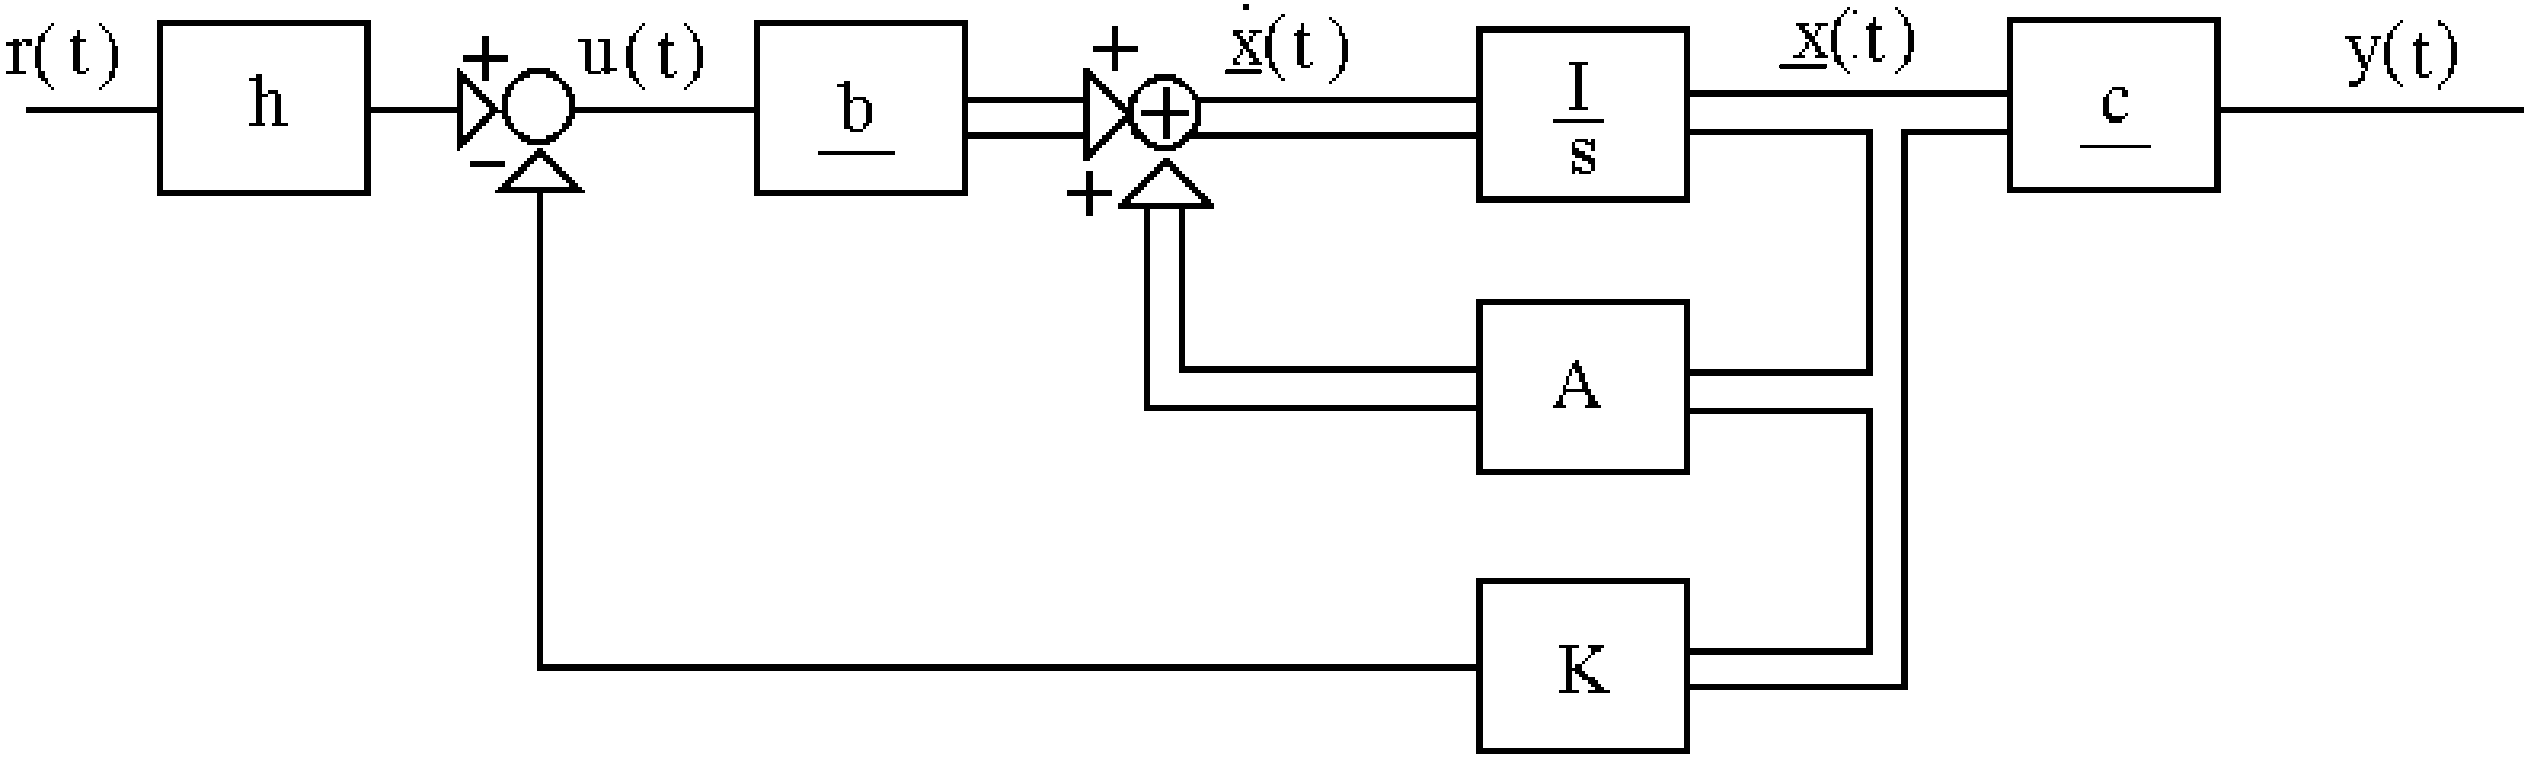
\includegraphics[width=\linewidth]{poleplacementPic.png}
 %\vspace*{-0.2cm}
\textbf{2. Tracking a Reference Signal}
 %\vspace*{-0.2cm}
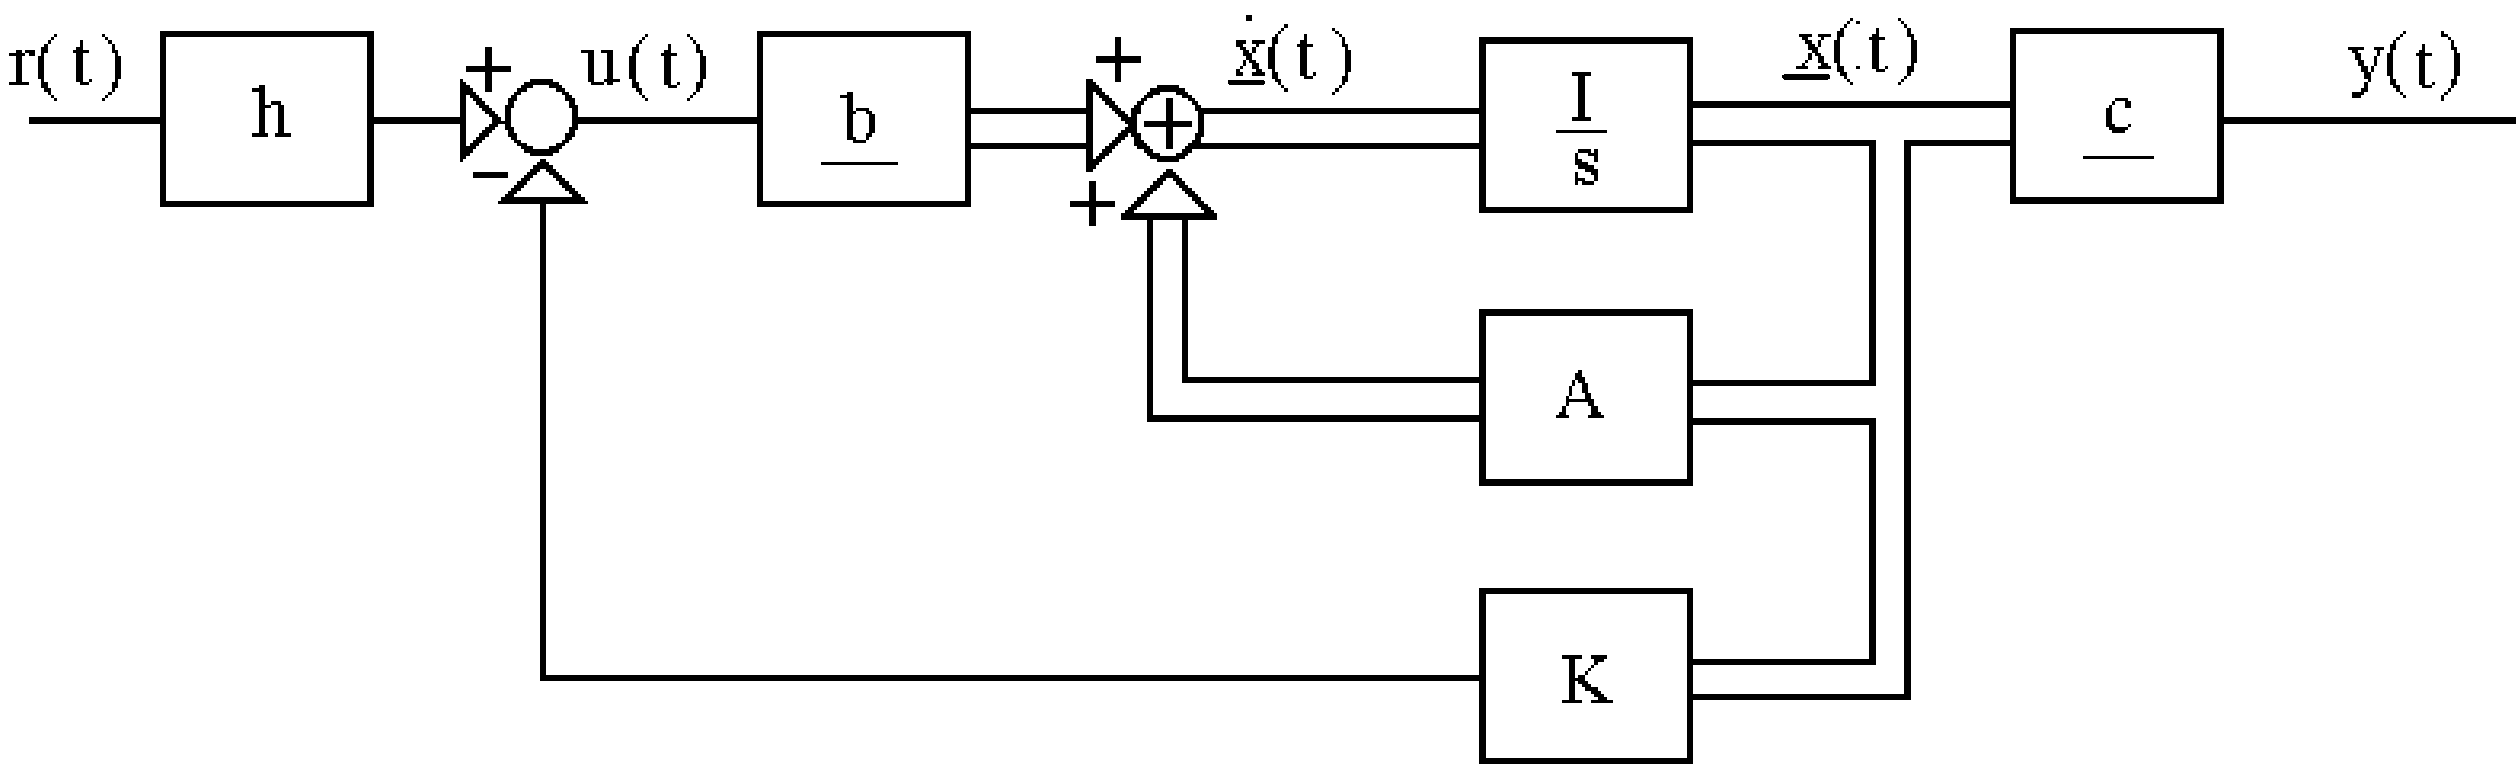
\includegraphics[width=\linewidth]{trackingRefSig.png}
\textbf{Tracking}: y(t) should follow r(t) at steady state(ss)
i.e, y(k) follows r(k) at ss. Find $h$ in $u(k)=hr(k) -Kx(k)$ for tracking. ss $x(k+1)=x(k)$
%\vspace*{-0.2cm}
\begin{align*}
& \dot{x}(t)=Ax+bu=x(t) \downarrow \\
& x(t)=(A-bK)x(t)+bhr(t) \\
& y(t)= c(I-G+HK)^{-1}Hr(t) \quad y(t)=r(t) \\
& h = \frac{-1}{c(A-bK)^{-1}b}
\end{align*}
Estimation of unmeasurable state variables is commonly called observation. $G(s)=C(sI-A)^{-1}B$,
 $\Delta (\lambda)= (\lambda^2+2\zeta \omega_n+ \omega_n^2)(\lambda + \zeta \omega_n)$ \hfill \break 
Overdamped $\zeta > 1$, Critically Damped $\zeta=1$, Underdamped(oscillations) $0< \zeta < 1$
$\zeta = \frac{-\ln(\% OS /100)}{\sqrt{\pi^2 + \ln^2(\% OS /100)}}$
$t_{s} = \frac {4}{\sigma } = \frac {4}{\zeta \omega _{n}}\ \left ( 2\%\ band \right )$,
$t_{s} = \frac {3}{\sigma } = \frac {3}{\zeta \omega _{n}}\ \left ( 5\%\ band \right )$,
% break to make column
\columnbreak
\textbf{Discretization of CTS-Time State Equations:}
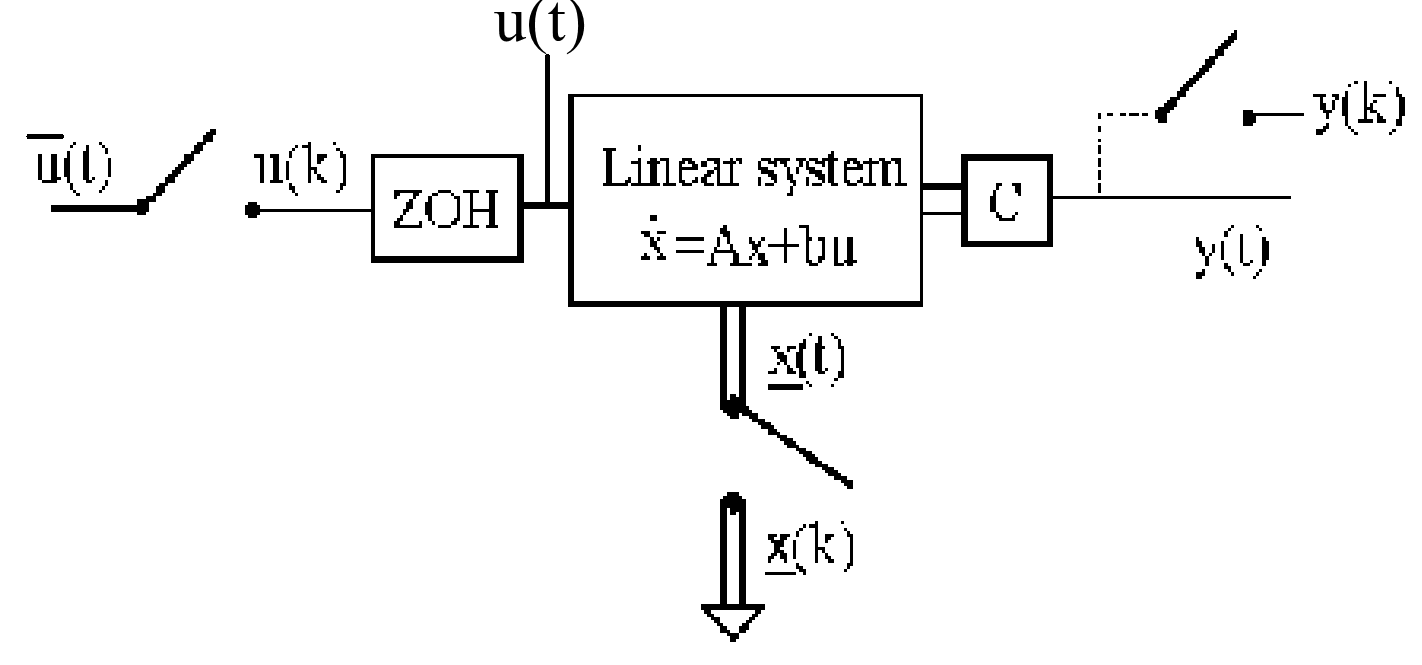
\includegraphics[width=\linewidth]{dis2CTS.png}
%\vspace*{-1.1cm}
\begin{align*}
&  \dot{x}=Ax+bu \quad G(T)=e^{AT}= \phi(T) \ H(T) = (\int_0^T e^{AT} \ dt)b
\end{align*}
%\vspace*{-0.6cm}
\textbf{3. Integral Error Feedback Discrete}
%\vspace*{-0.05cm}
$
x(k+1)=Gx(k)+Hu(k)+w(k) \quad y(k)=c(k)x(k) 
$
w(k) is unknown but constant disturbance.

Problem: Design a state-feedback controller so that
1) The CL eigenvalues are at prescribed locations.

2) The output y(k) follows the reference r(k) for any w(k)
(constant, but unknown) at steady state.

$
 \begin{bmatrix} x(k+1) \\ q(k+1)\end{bmatrix} =
\begin{bmatrix}G & 0 \\ -T_c & 1\end{bmatrix}\begin{bmatrix}x(k) \\ q(k)\end{bmatrix}+
\begin{bmatrix}H \\ 0\end{bmatrix}u(k)+\begin{bmatrix} 0 \\ T\end{bmatrix}r(k)+\begin{bmatrix}w(k) \\ 0\end{bmatrix} \ \
q(k+1)=q(k)+T(r(k)-y(k)) 
$

Find $K = [K_x, K_q]$,$K=(\alpha-a)\tilde{A}^{-T}C^{-1}$,

$ \begin{bmatrix} x(k+1) \\ q(k+1)\end{bmatrix} =
\begin{bmatrix}G-HK_x & -HK_q \\ -T_c & 1\end{bmatrix}\begin{bmatrix}x(k) \\ q(k)\end{bmatrix}+
\begin{bmatrix}0 \\ T\end{bmatrix}u(k)+\begin{bmatrix} 0 \\ T\end{bmatrix}r(k)+\begin{bmatrix}w(k) \\ 0\end{bmatrix}$ $u(k)=-[K_x, K_q]\begin{bmatrix} x(k) \\ q(k)
\end{bmatrix}$ %\hfill \break %using a(z) as given  given characteristic polynomial, and $\alpha(z)$ as desired ch. eqn. \hfill \break 
%\begin{minipage}[h]{1\linewidth}
%\textbf{Discrete} \hfill \break 


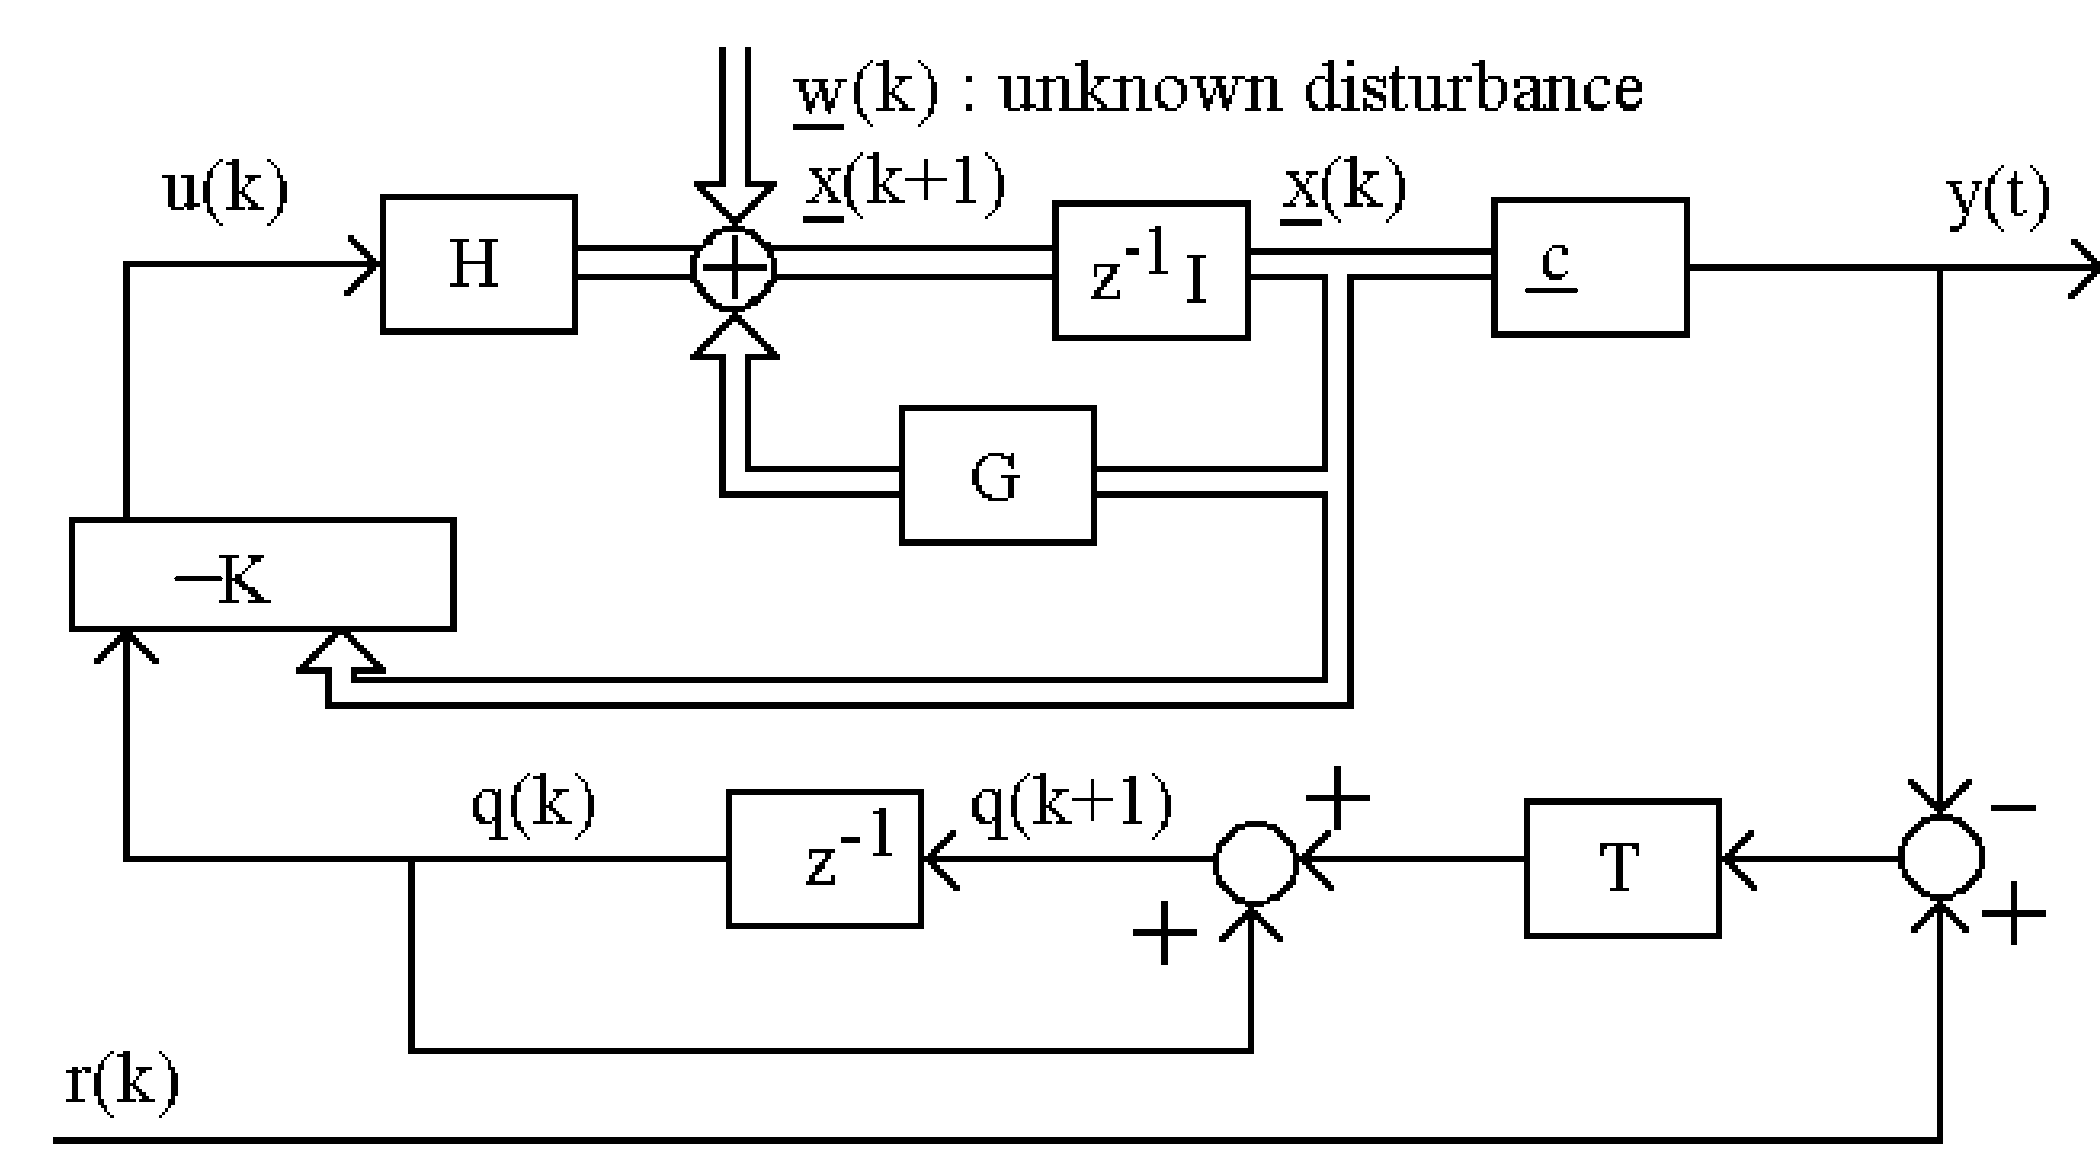
\includegraphics[width=\linewidth]{DiscreteIntegralTracking.png}
%\end{minipage}
%\begin{minipage}[h]{1\linewidth}
%\textbf{Continuous}
\textbf{3. Integral Error Feedback CTS} 

$ \begin{bmatrix} x(k+1) \\ q(k+1)\end{bmatrix} =
\begin{bmatrix}A & 0 \\ -c & 1\end{bmatrix}\begin{bmatrix}x(k) \\ q(k)\end{bmatrix}+
\begin{bmatrix}b \\ 0\end{bmatrix}u(k)+\begin{bmatrix} 0 \\ 1\end{bmatrix}r(k)+\begin{bmatrix}w(k) \\ 0\end{bmatrix} \ \
q(k)=(r(k)-y(k)) $
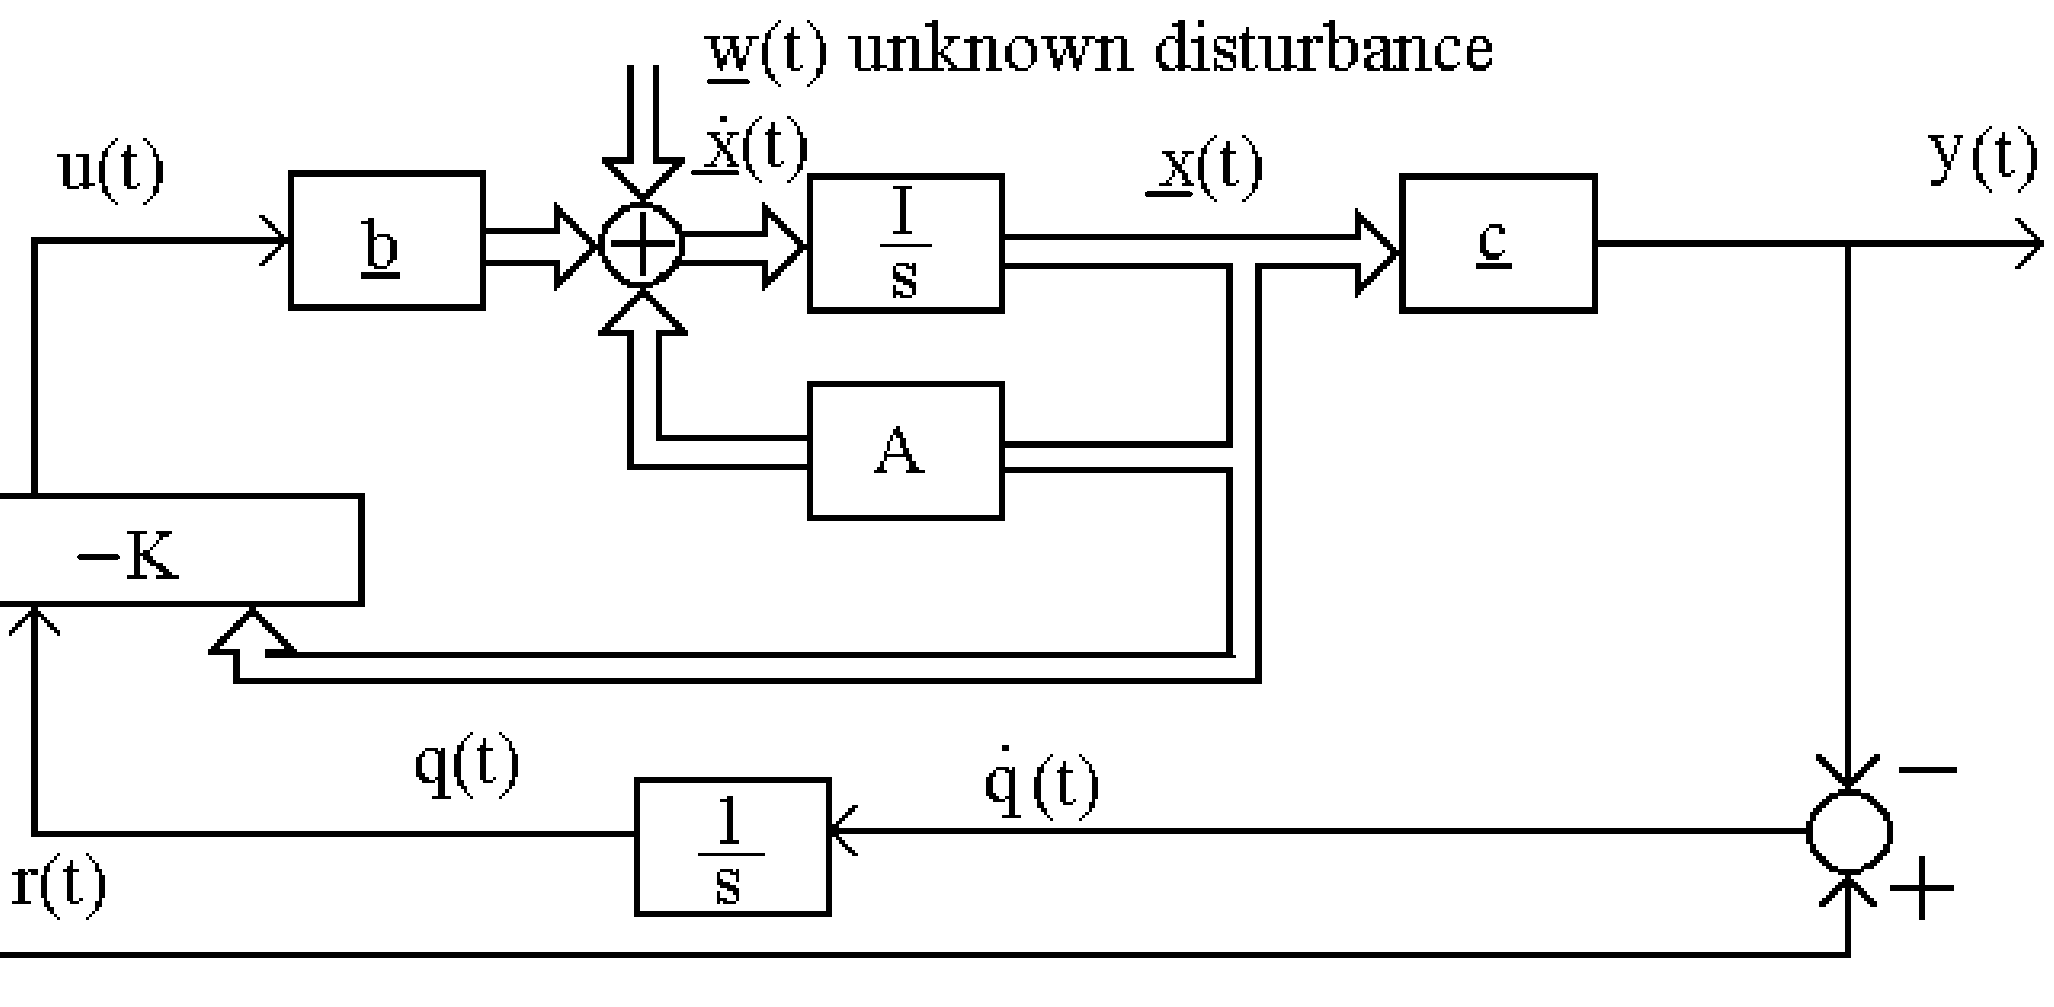
\includegraphics[width=\linewidth]{CTSIntegralTracking.png}
%\end{minipage}
\textbf{Combined Observer-Controller}

Observer feedback: $l(y(t)-c\tilde{x}(t))$,

Feedback control signal $u(t)=-K\tilde{x}(t)+v(t)$ \hfill \break 
Observation error: $\dot{e}(t)=(A-lc)e(t)$
$\det \begin{bmatrix}sI-A & bK \\
-lc & sI-A+lc+bK
\end{bmatrix} \\ =\det(sI-A+bk)\det(sI-A+lc)$
$\begin{bmatrix}
\dot{x}(t) \\
\dot{\tilde{x}}(t)
\end{bmatrix}= \begin{bmatrix}
A  & -bK \\
lc & A-lc-bK
\end{bmatrix}\begin{bmatrix}
x(t) \\
{\tilde{x}}(t)
\end{bmatrix}+
\begin{bmatrix}
b \\ b
\end{bmatrix} v(t) \quad 
\begin{bmatrix}
x(t_0) \\ \tilde{x}(t_0)
\end{bmatrix}=
\begin{bmatrix}
x_0 \\ \tilde{x}_0
\end{bmatrix}
$
\vspace{0.1 cm}
Quad Form: $ax^2+bx+c=0 \quad x= \frac{-b \pm \sqrt{b^2-4ac}}{2a}$,
Steady-state error is defined as the difference between the input (command) and the output of a system in the limit as time goes to infinity. $x_1(1)=x_2(0)$.
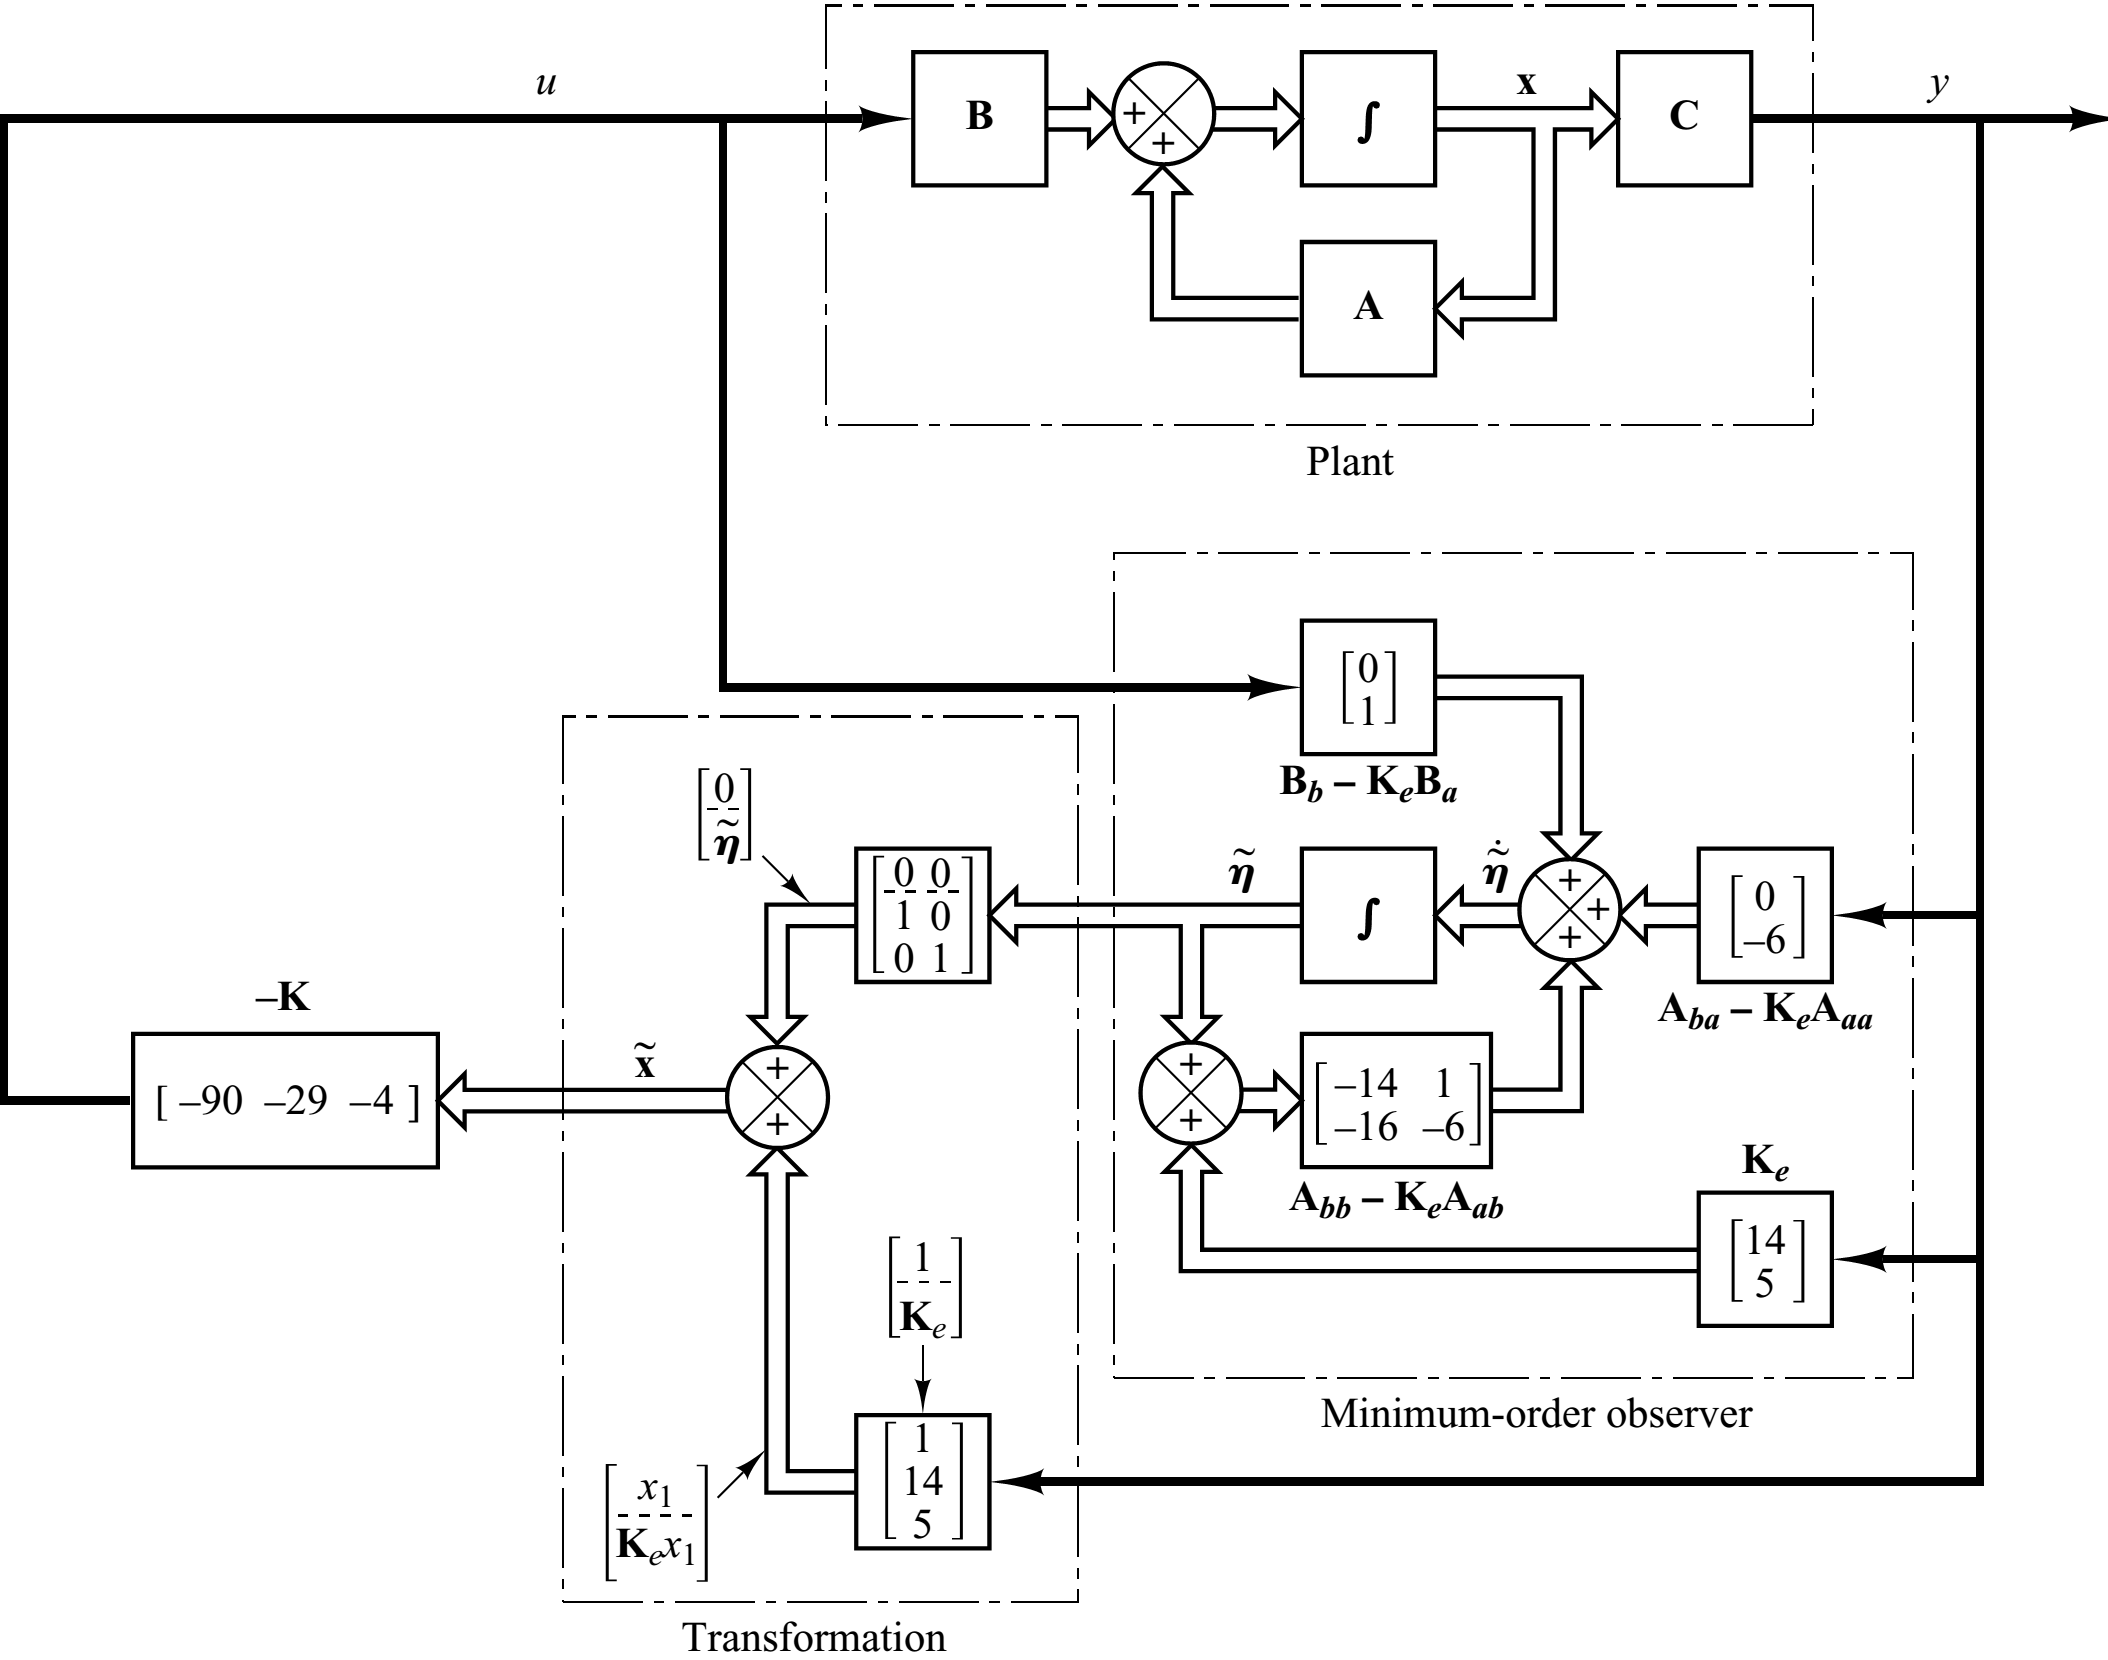
\includegraphics[width=\linewidth]{fullEstimateobs.png}
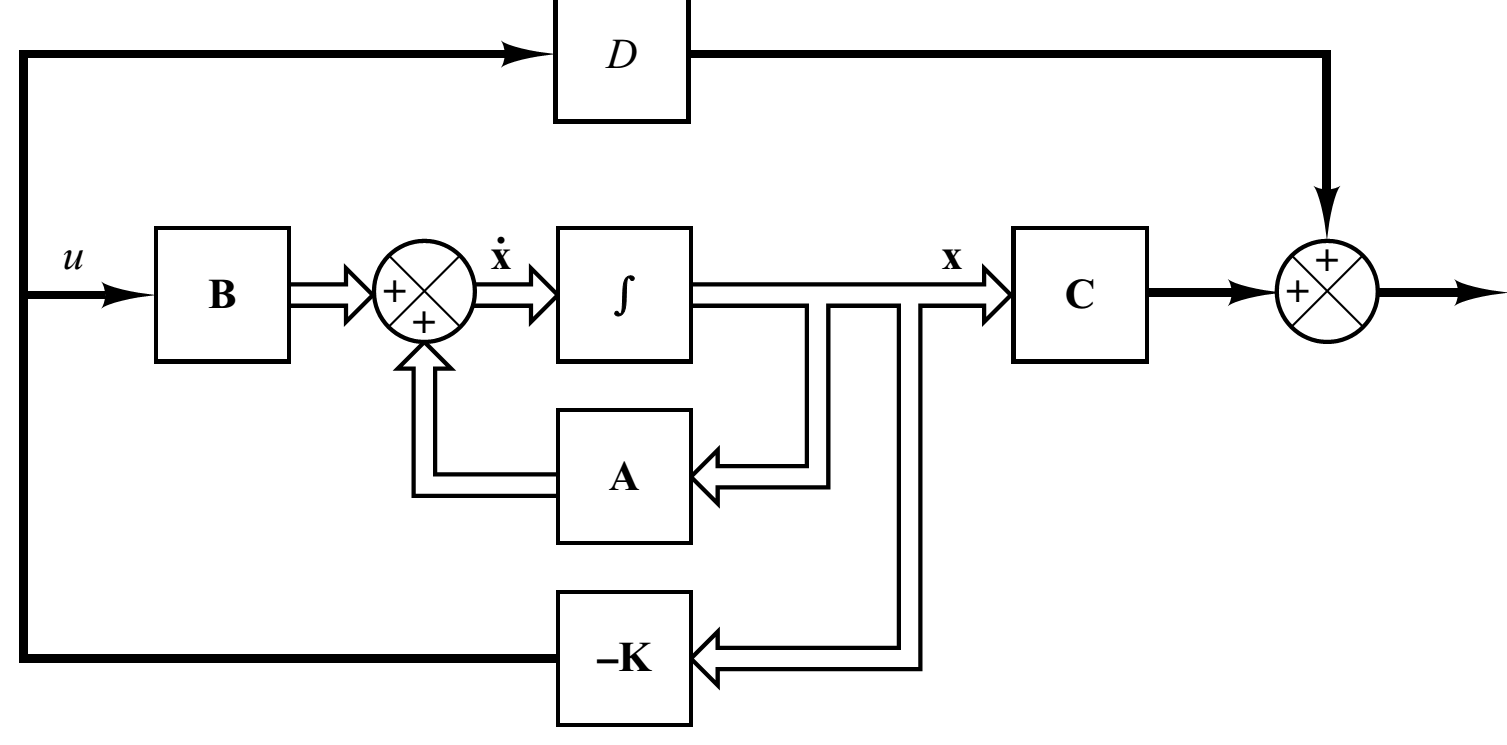
\includegraphics[width=\linewidth]{keFeedback.png}
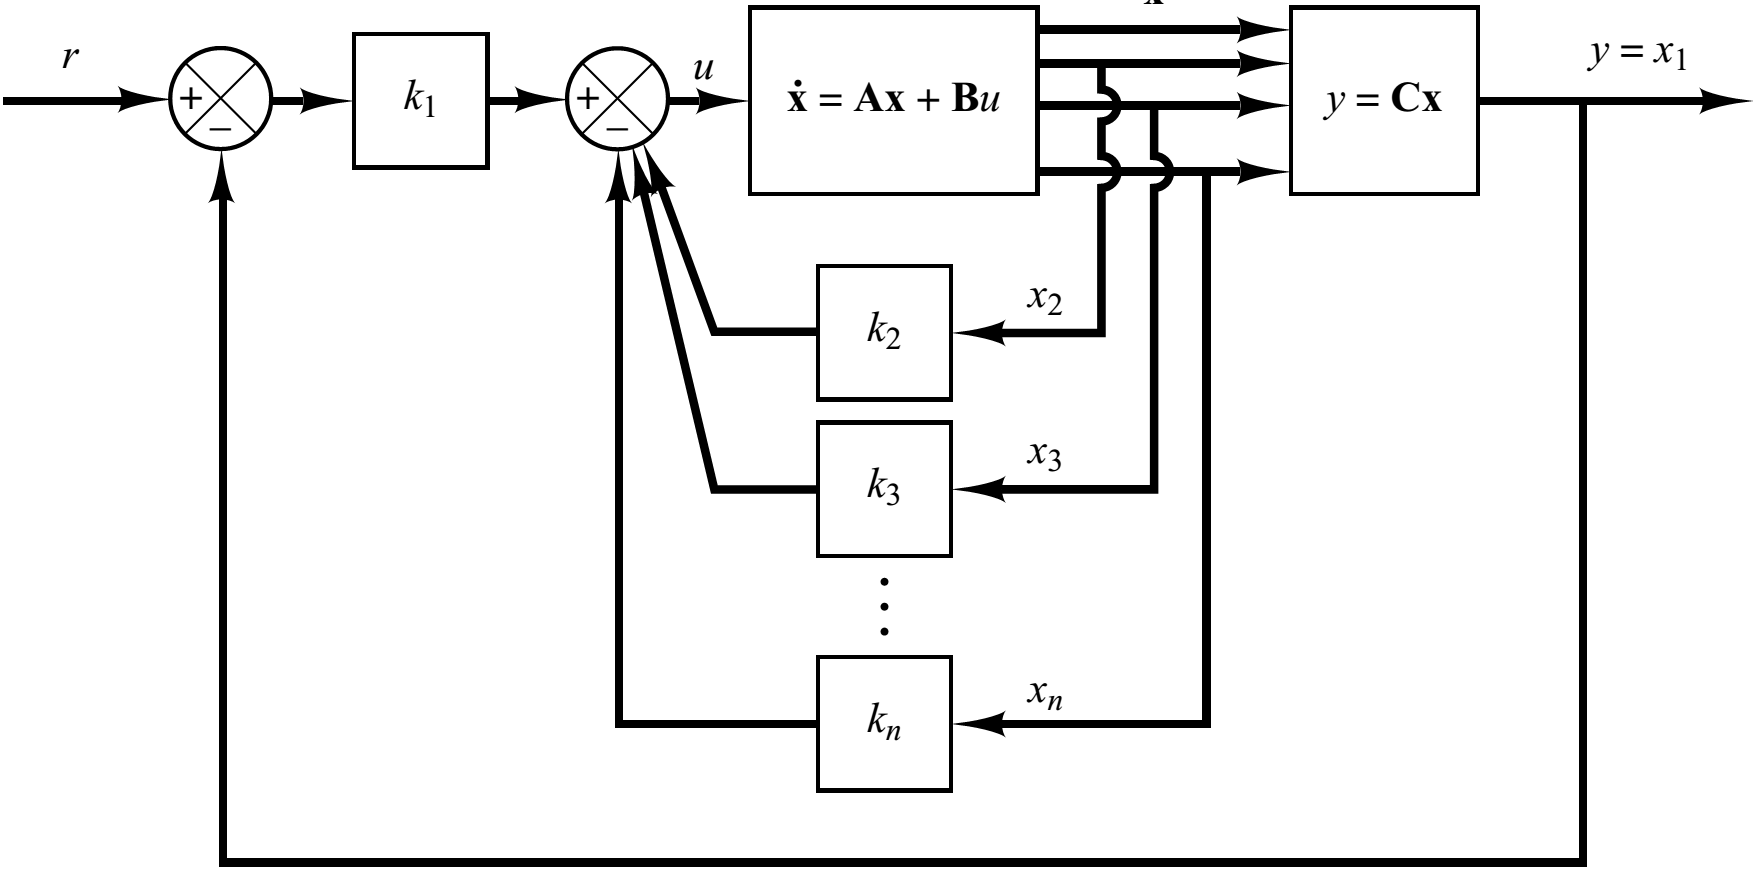
\includegraphics[width=\linewidth]{whyNot.png}
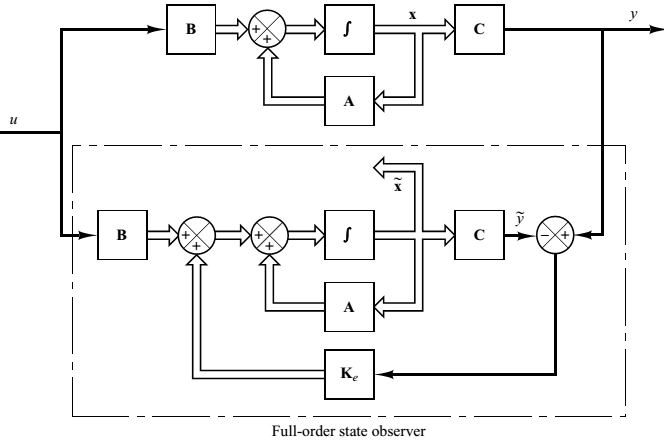
\includegraphics[width=\linewidth]{full-state-obs.png}
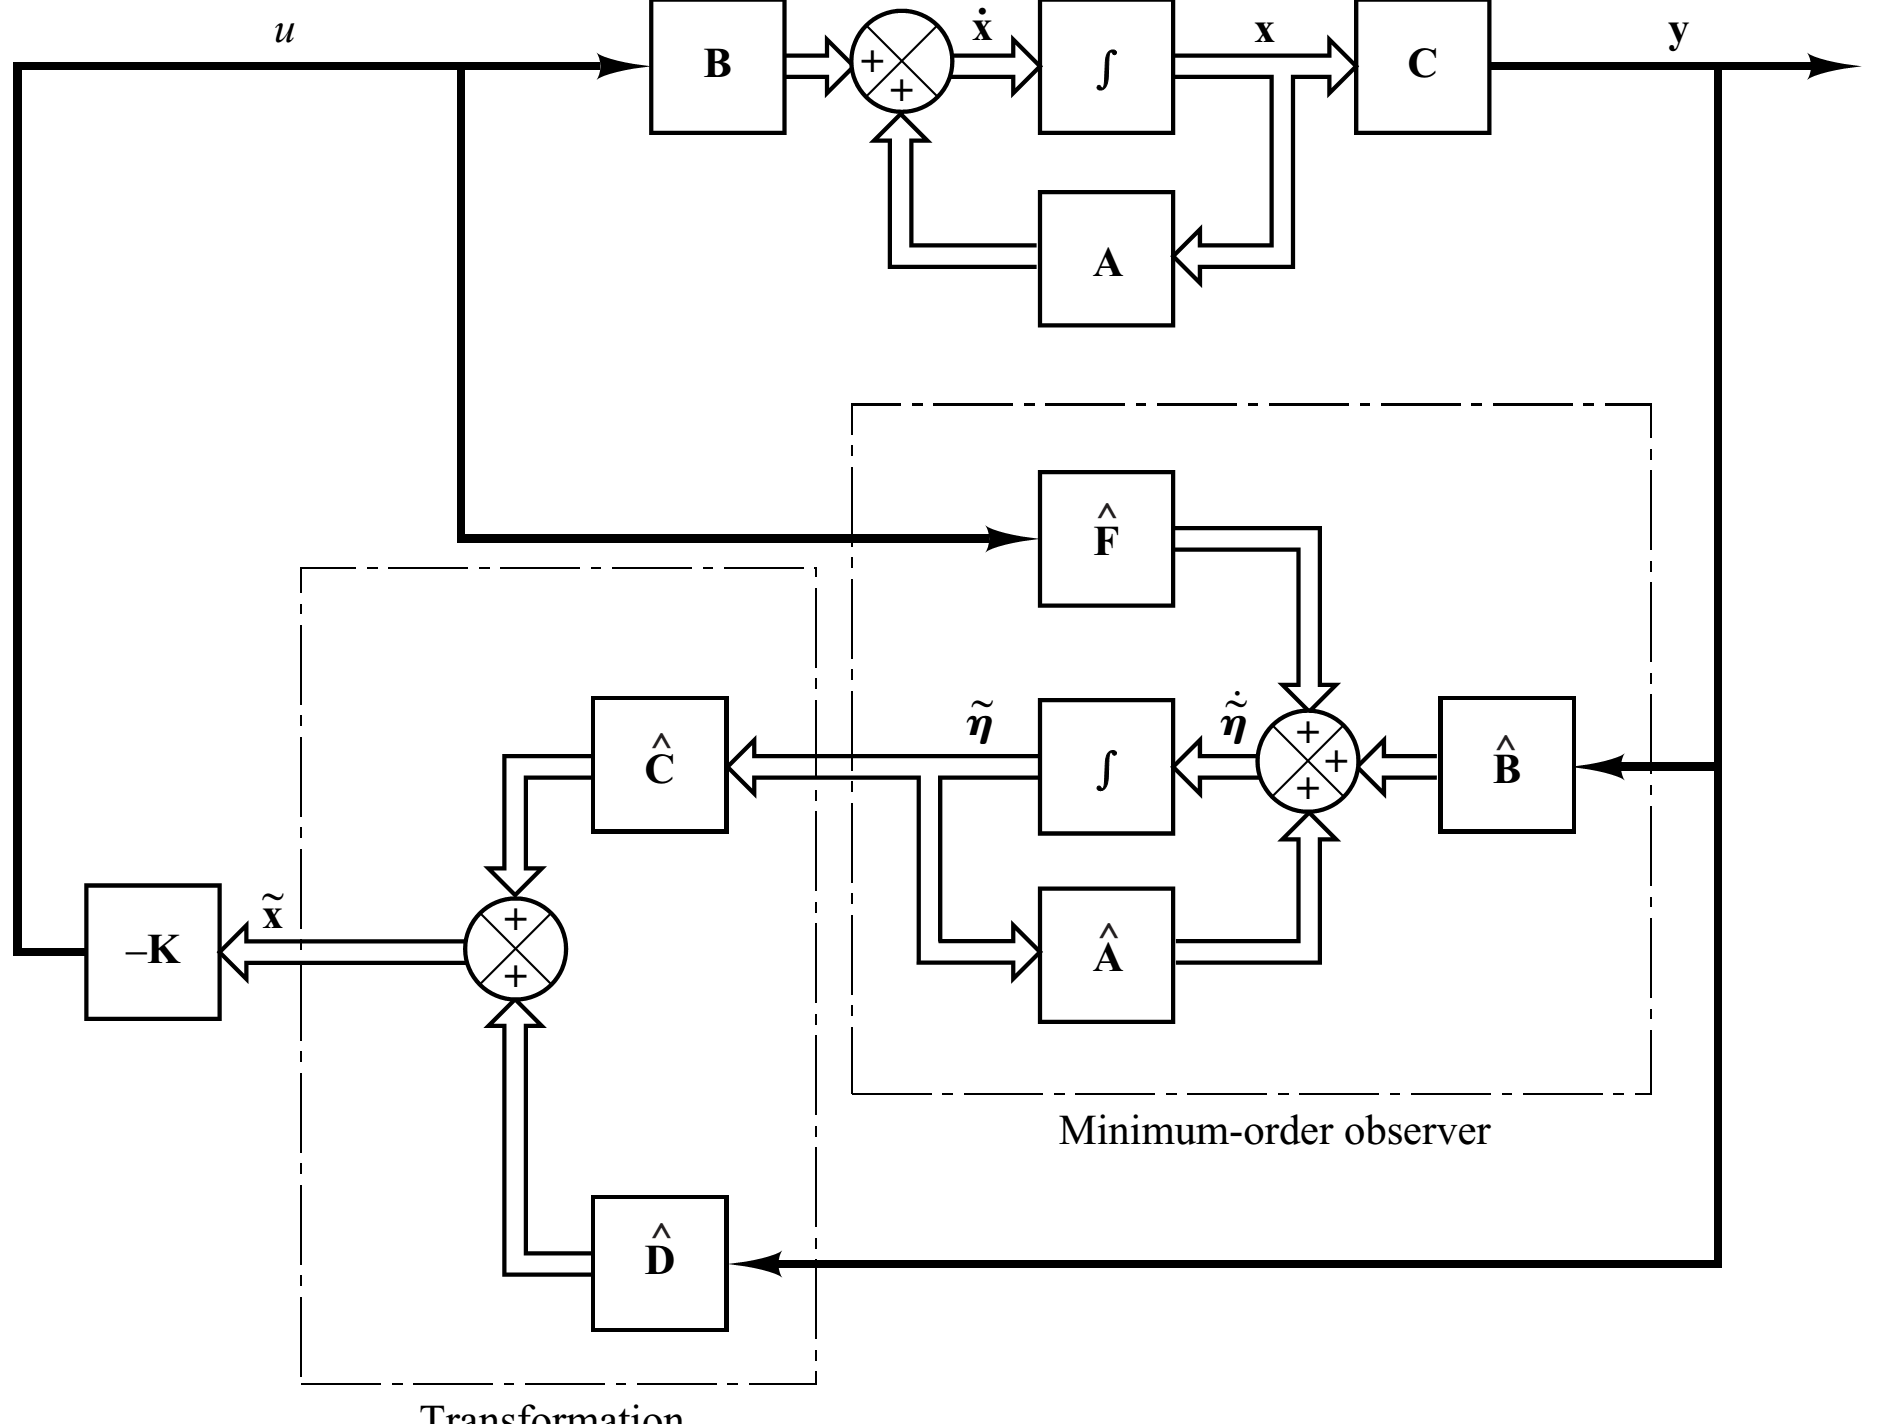
\includegraphics[width=\linewidth]{min-order-observer.png}




\subsection{Stability Test for Digital Systems}

\textbf{Jury-Marden Table Uses function P of z} \newline
%\vspace*{-0.25cm}
\begin{align*}
& b_k = \det \begin{bmatrix}
a_n & a_{n-1-k} \\
a_0 & a_{k+1}
\end{bmatrix} \\
& k = 0,1,  \cdots n-1 \\
& c_k = \det \begin{bmatrix}
b_{n-1} & b_{n-2-k} \\
b_0 & b_{k+1}
\end{bmatrix} \\
& k = 0,1,  \cdots n-1 \\
& q_k = \det \begin{bmatrix}
p_{3} & p_{2-k} \\
p_0 & p_{k+1}
\end{bmatrix} \\
& k =0,1,2
\end{align*}

\begin{tabular}{llllllll}
	\cline{1-5}
	Row & $z^0$     & $z^1$     & $z^2$     &          & $z^{n-2}$ & $z^{n-1}$ & $z^n$ \\ %\cline{1-5}
	1   & $a_n$     & $a_{n-1}$ & $a_{n-2}$ & $\cdots$ & $a_2$     & $a_1$     & $a_0$ \\
	2   & $a_0$     & $a_1$     & $a_2$     & $\cdots$ & $a_{n-2}$ & $a_{n-1}$ & $a_n$ \\
	3   & $b_{n-1}$ & $b_{n-2}$ & $b_{n-3}$ & $\cdots$ & $b_1$     & $b_0$     &       \\ %\cline{1-5}
	4   & $b_0$     & $b_1$     & $b_2$     & $\cdots$ & $b_{n-2}$ & $b_{n-1}$ &       \\
	5   & $c_{n-2}$ & $c_{n-3}$ & $c_{n-4}$ & $\cdots$ & $c_0$     &           &       \\
	6   & $c_0$     & $c_1$     & $c_2$     & $\cdots$ & $c_{n-2}$ &           &      \\
	2n-5& $p_3$ & $p_2$ & $p_1$ & $p_0$ & & & \\
	2n-4& $p_0$ & $p_1$ & $p_2$ & $p_3$ & & & \\
	2n-3& $q_2$ & $q_1$ & $q_0$ & & & & 
\end{tabular}

\begin{align*}
& P(z) = a_0z^n+a_1z^{n-1} + \cdots + a_{n-1}z+a_n \quad G(z)= \frac{A(z)}{P(z)} \\
& \text{Stability Condition:} \quad P(z) \neq 0 \quad |z| \geq 1 \quad (\text{Draw Unit Circle to test stability})\\
& \text{Routh-Stability in Digital Domain: } s = \frac{z+1}{z-1} \quad z=\frac{s+1}{s-1}
\end{align*}


\begin{align*}
& G(z) = \mathcal{Z} \left\{\left(\frac{1-e^{-s}}{s}\right) \left[ \frac{1}{s+1}\right] \left[\frac{1}{s}\right] \right\} \rightarrow G_1(z) = (1-z^{-1})\mathcal{Z} \left\{ \frac{1}{s^2(s+1)} \right\}
\end{align*}

All first-column elements of the Routh array are to be of the same sign. $a_0s^n + a_1s^{n-1}+ \cdots + a{n-1} s + a_n = 0$, first row is even entries $a_0$, $a_2$, next row is $a_1$, $a_2$, b entries are the same are jury-marden table.


\subsection{Z-transform}



\begin{tabular}{c c}
	$\mathcal{Z} \left\{ f_1(t) \pm f_2(t) \right\}=F_1(z)+F_2(z)$ & Addition\\
	$\mathcal{Z} \left\{ af(t) \right\}= aF(z)$ & Multiplication by a Constant \\
	$\mathcal{Z} \left\{ f(t-nT) \right\}=z^{-n}F(z)$ & Shifting \\
	$\mathcal{Z} \left\{ f(t+kT) \right\}=z^{k}F(z)-z^{k}f(0)- \cdots - z f(kT-T)$ & Shifting (cont'd) \\
	$\mathcal{Z} \left\{ e^{\mp at} f(t) \right\}=F(ze^{\pm at})$ & Complex Translation \\
	$\lim_{k \rightarrow \infty} f(kT)= \lim_{z \rightarrow 0}F(z)$ & Initial Value Theorem \\ 
	If $(1-z^{-1})F(z)$ has all singularities inside unit disk $|z|=1$, then & Final Value Theorem \\
	$\lim_{k \rightarrow \infty} f(kT) = \lim_{z \rightarrow 1} (1-z^{-1})F(z)$ & \\
	$\mathcal{Z} \left\{ \frac{\partial}{\partial a} f(t,a) \right\} = \frac{\partial}{\partial a} F(z,a)$ & Partial differentiation
\end{tabular}




    
\end{document}